\documentclass[oneside,final,12pt]{extreport}
%should it be twoside or oneside??
\usepackage[utf8]{inputenc}
\usepackage[russianb]{babel}
\usepackage{vmargin}
\setpapersize{A4}
%   left, top, right, bottom, headers/footers(3), page number
\setmarginsrb{3cm}{2cm}{1.5cm}{2cm}{0pt}{0mm}{0pt}{13mm}
\fussy
%\sloppy
\usepackage{indentfirst}

\usepackage{graphicx}
\usepackage{amsmath,amsfonts,amssymb,amsthm,mathtools}
\usepackage{siunitx}
\usepackage{physics}
\usepackage{hyperref}

\usepackage[labelsep=endash]{caption}
\addto\captionsrussian{\renewcommand{\figurename}{Рисунок}}
\addto\captionsrussian{\renewcommand{\tablename}{Таблица}}

% \renewcommand{\thesection}{\arabic{section}} % remove 0. prefix
\newcommand\Section[1]{
  \refstepcounter{section}
  \section*{\centering
    \arabic{section}. #1}
  \addcontentsline{toc}{section}{%
    \arabic{section}. #1}
}
\newcommand\Subsection[1]{
  \refstepcounter{subsection}
  \subsection*{\centering
    \arabic{section}.\arabic{subsection}. #1}
  \addcontentsline{toc}{subsection}{%
    \arabic{section}.\arabic{subsection}. #1}
}



\begin{document}

\begin{titlepage}

Титульник.

\end{titlepage}
\setcounter{page}{2}

\section*{Аннотация.}
% Цели и задачи. Результаты. Рекомендации, предложенные на основании работы.
Целью данной работы является освоение пакета программ
COMSOL Multiphysics\texttrademark\ в целях
математического моделирования процессов массопереноса в микрофлюидных системах.
Для этого были смоделированы:
\begin{itemize}
  \item специфическое связывание аналита с:
    \begin{itemize}
      \item модифицированной поверхностью в канале, через который протекает раствор,
      % \item модифицированной мембраной, через которую протекает раствор
      \item модифицированной поверхностью микросфер, находящихся в растворе;

    \end{itemize}

  % \item несколько пассивных микрофлюидных каплегенераторов.
    % список каплегенераторов?

\end{itemize}

С помощью данных моделей удалось:
\begin{itemize}
  \item найти значение безразмерного коэффициента,
    позволяющее понизить размерность (с 2 до 1) задачи об адсорбции на
    поверхность канала,
  % \item обнаружить влияние учёта массопереноса в области пространства
  %   за пределами диффузионного слоя в задаче об адсорбции на поверхность канала,
  \item показать, что одномерный вариант задачи об адсорбции на поверхности канала
    пригоден для моделирования отмывки от неспецифически связавшегося с поверхностью вещества.

\end{itemize}



\tableofcontents

\clearpage

\Section{Обозначения и сокращения}
\begin{description}
  \item[УрЧП:] уравнение в частных производных, уравнение математической физики.
%   \item[Диагностическе системы:]
  \item[(Не)специфическая адсорбция:] (не)специфическое связывание
    молекулы из раствора с молекулой на поверхности или с самой поверхностью,
    НЕ имеется в виду разница между адсорбцией, обусловленной
    электростатическим притяжением иона к поверхности
    и обусловленной силами Ван-дер-Ваальса.
  \item[Уравнение:] под уравнением зачастую имеется в виду система уравнений.

\end{description}

\Section{Введение}
% Новизна, актуальность, цели и задачи.
Микрофлюидика --- научно-инженерная область, посвящённая поведению
малых объёмов жидкости при малых потоках.
Микрофлюидика применяестя в биологии, медицине и нанотехнологиях.

В связи с малыми размерами микрофлюидных систем, их поведение не интуитивно,
а наблюдения за состоянием и поведением таких систем затруднены.
Из-за этого в микрофлюидной практике
для создания систем с предсказуемыми свойствами (и для других целей)
применяется математическое моделирование.
Для этих целей широко применяется пакет программ COMSOL Multiphysics\texttrademark{}
(далее COMSOL).

Целью работы является освоение COMSOL.
Задачи работы:
\begin{itemize}
  \item создание моделей специфического связывания аналита с:
    \begin{itemize}
      \item модифицированной поверхностью канала, через который протекает раствор аналита:
        в двумерной и одномерной постановках,
        при наличии и отсутствии неспецифически связывающихся молекул в растворе,
        при наличии и отсутствии сайтов неспецифического связывания на поверхности;
      % \item модифицированной мембраной, через которую протекает раствор аналита:
      %   в предположении, что мембрана является областью пространства,
      %   где сайты связывания распределены равномерно, и
      %   в предположении, что мембрана является набором нитей разных форм,
      %   расположенных параллельно, на поверхности которых располагаются сайты связывания;
      \item модифицированной поверхностью микросфер, находящихся в растворе аналита:
        находящихся в потоке и при отсутствии течения.

    \end{itemize}

  % \item создание моделей пассивных каплегенераторов

\end{itemize}

\Section{Обзор литературы}

\Subsection{Микрофабрикация}
Микрофабрикация --- научная и инженерная область, посвящённая созданию
миниатюрных изделий со сложной геометрией. Изначально микрофабрикация была
связана с созданием полупроводниковых микросхем малых размеров,
высоких производительности и надёжности.

Методы микрофабрикации оказались применимы для создания микрофлюидных систем,
как правило, называемых микрофлюидными чипами (или просто чипами для краткости),
полезных для био-медицинского направления и не только.

Основные средства микрофабрикации --- различные виды литографии.
% TODO поперечислять виды и возможности


\Subsection{Микрофлюидика}

Микрофлюидика --- наука о поведении малых объёмов жидкостей (от микро- до фемтолитров)
при малых потоках.
Малость объёмов и потоков можно определять значимостью эффектов масштаба:
ламинарные потоки, определяющая роль капиллярных явлений.

Микрофлюидика применяется\cite{bib:fabrication_and_application}:
\begin{itemize}
  \item для создания диагностических систем (\textbf{lab-on-a-chip})
        (рис.~\ref{fig:diagnostic_example}),

  \item для создания и исследования культур клеток (\textbf{organ-on-a-chip}),

  \item для адресной доставки лекарственных веществ (drug delivery),

  \item для синтеза наноматериалов.

\end{itemize}

\begin{figure}[h]
  \centering
  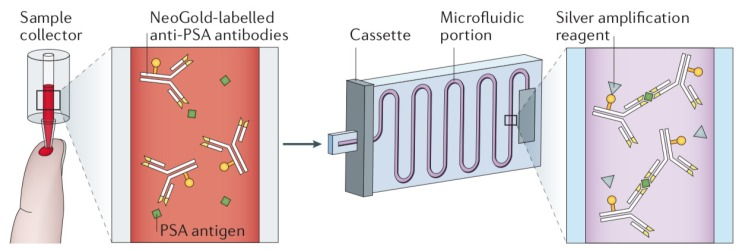
\includegraphics[width=.7\textwidth]{pic/diagnostic_device_example}
  \caption{\label{fig:diagnostic_example}%
    Пример микрофлюидной диагностической системы из~\cite{bib:PoC_trends},
    пригодной для обнаружения простатического специфического антигена (ПСА)
    менее, чем за 15 минут
    % за менее чем 15 минут
  }

\end{figure}
% \FloatBarrier{}

Для данной работы интерес представляют, в первую очередь,
диагностические системы.
Диагностическими здесь и далее называются системы, позволяющие обнаружить
(по возможности, определить/оценить количественно)
содержание конкретного вещества в некотором растворе
(зачастую --- в биологической жидкости, например, в крови, моче, слюне, лимфе и т. д.)
К возможным преимуществам использования
микрофлюидных диагностических систем относятся:
\begin{itemize}
  \item работа с малыми объёмами исследуемой жидкости,

  \item использование малых количеств веществ-детекторов,

  \item минимизация потерь жидкости на стенках реактора в виду отсутствия
    необходимости переноса веществ между сосудами,

  \item увеличенная скорость диффузионного массопереноса,

  \item портативность,

  \item простота в использовании.

\end{itemize}
Последние два пункта являются ключевыми для создания диагностических устройств,
которые можно использовать вдали от оснащённых лабораторий и
квалифицированных специалистов
(\textbf{PoC} (point-of-care) devices).

Далее будем подразумевать, что ключом к детекции так или иначе
является специфическая адсорбция аналита,
что исключает из числа рассматриваемых диагностических методик, например, ПЦР.


% TODO больше микрофлюидики богу микрофлюидики
% TODO uTAS, электрофорез и хроматография
% TODO добавить описания/примеры/возможности диагностических микрофлюидных систем
% TODO элементы микрофлюидных систем


\Subsection{Математическое описание релевантных физическо-химических процессов}

\subsubsection*{Основная система уравнений}
Течение жидкости в микрофлюидных системах характеризуется малыми числами
Рейнольдса, т. е. поток в микроканалах можно считать ламинарным.
Жидкость можно считать несжимаемой, что приводит к системе уравнений
\begin{equation}
\begin{cases}
  \rho\frac{\displaystyle \partial \vb v}{\displaystyle \partial t} = -\nabla P + \eta\Delta\vb v + \vb f
    & \left(\text{уравнение Стокса}\right) \\
  \nabla\cdot\vb v = 0 & \left(\text{несжимаемость}\right) \\
  \frac{\displaystyle \partial c_i}{\displaystyle \partial t} = -\nabla\cdot\vb j_i + R_i
    & \left(\text{массоперенос}+\text{химия}\right) \\
  \vb j_i = -D_i\nabla c_i + c_i \vb v
    & \left(\text{конвекция-диффузия}\right) \\
\end{cases}
\label{eq:main}
\end{equation}
где $\rho$ --- плотность раствора $\left[\text{г}/\text{мл}\right]$,
$\vb v$ --- скорость ламинарного течения $\left[\text{мм}/\text{с}\right]$,
$P$ --- гидростатическое давление $\left[\text{Па}\right]$,
$\eta$ --- динамическая вязковть раствора $\left[\text{Па}\cdot\text{с}\right]$,
$\vb f$ --- внешняя сила, действующая на элемент объёма раствора
$\left[\text{дина}/\text{мл}\right]$
(например, сила тяжетси),
$c_i$ --- концентрация $i$-ого вещества в растворе $\left[\text{мМ}\right]$,
$\vb j_i$ --- поток $i$-ого вещества в растворе
$\left[\text{мМ}/\left(\text{мм}^2\cdot\text{с}\right)\right]$,
$R_i$ --- изменение концентрации $i$-ого вещества в растворе, связанное с
химическими реакциями $\left[\text{мМ}/\text{с}\right]$.

По всей видимости, (существенных для микрофлюидики) границ применимости
у системы~\eqref{eq:main} две:
\begin{enumerate}
  \item концентрации растворённых веществ должны быть достаточно большими,
    чтобы было допустимым не переходить к статистическому описанию
    движения их молекул, а остаться в рамках непрерывного приближения,
    % TODO а что с очент большими концентрациями???

  \item характерный размер $\lambda$ (ширина) микрофлюидного канала должнен
    значительно превосходить длины
    свободного пробега молекул, чтобы течение жидкости было вязкостным,
    а не переходным или молекулярным (Кнудсеновским);
    на практике, для водоподобный сред, это ограничение
    $\lambda\gtrsim300\text{нм}$.

\end{enumerate}

\subsubsection*{Граничные условия}
Далее приняты следующие обозначения: $\Omega$ --- расчётная область,
$\mathcal{W} \subset \partial\Omega$ --- стенка
(на ней обнуляется скорость течения),
$\mathcal{S}_i \subset \mathcal{W}$ --- часть стенки,
содержащая сайты связывания $i$-ого вещества,
$\mathcal{I} \subset \partial\Omega$ --- входное отверстие (inlet),
$\mathcal{O} \subset \partial\Omega$ --- выходное отверстие (outlet).

Граничные условия для системы~\eqref{eq:main} на стенке $\mathcal{W}$:
\begin{equation}
\begin{cases}
  \left. \vb v \right|_{\mathcal{W}} = \vb 0 \\
  \left. \vb n \cdot \vb j_i \right|_{\mathcal{W}} = r_i\chi_{\mathcal{S}_i}
\end{cases}
\label{eq:main:bc_walls}
\end{equation}
где $r_i$ --- скорость адсорбции $i$-ого вещества,
$\chi_{\mathcal{S}_i}$ --- характеристическая функция части стенок,
на которой адсорбция вообще происходит,
$\vb n$ --- поле единичных внешних нормалей к $\partial \Omega$.
Такое описание несколько избыточно: действительно, можно сделать замену
$r_i = r_i\chi_{\mathcal{S}_i}$.

Граничные условия на входном/выходном отверстиях $\mathcal{I}$/$\mathcal{O}$:
\begin{equation}
\begin{cases}
  \left. \vb v \right|_{\mathcal{I}/\mathcal{O}}\left(t, x, y, z\right) \\
  \left. P \right|_{\mathcal{I}/\mathcal{O}}\left(t, x, y, z\right) \\
  \left. c_i \right|_{\mathcal{I}}\left(t, x, y, z\right) \\
  \left. \vb n \cdot \nabla c_i \right|_{\mathcal{O}} = 0 \\
\end{cases}
\label{eq:main:bc_io}
\end{equation}
здесь отсутствие правой части равенства подразумевает, что зафиксирована
(известна) <<стоящая в левой части равенства>> функция.


\subsubsection*{Изотермы адсорбции}
Под изотермой адсорбции будем понимать всякое уравнение
$F\left(c_{i=\overline{1,n}}, \gamma_{i=\overline{1,n}}\right) = 0$, где
$c_i$ --- равновесная концентрация $i$-ого вещества в растворе,
$\gamma_i$ --- равновесная (поверхностная) концентрация $i$-ого вещества
на поверхности, или параметрические семейства таких уравнений,
параметрами в которых будут такие величины как
поверхностная концентрация сайтов связывания и
равновесные химические константы (например, константа диссоциации).
Дополнительно потребуем, чтобы такие уравнения задавали функции
$\gamma_i\left(c_{i=\overline{1,n}}, \gamma_{j\neq i}\right)$.

Изотермы адсорбции здесь представляют интерес с точки зрения получения
выражений для скоростей реакций $r_i$ в
граничных условиях~\eqref{eq:main:bc_walls}.
Они также могут использоваться для приближений.

Простейшей (не считая изотерму адсорбции Генри) изотермой адсорбции является
изотерма \textbf{Ленгмюра} для одного вещества
с единственным видом сайтов связывания
с поверхностной концентрацией $\Gamma$
\begin{equation}
  \gamma = \frac{\Gamma c}{K_d + c},
\label{eq:Langmuir_single_eq}
\end{equation}
где $K_d$ --- константа диссоциации вещества и сайтов связывания на поверхности.
Изотерме Ленгмюра соответствует кинетика, описываемая законом действующих масс
% TODO закон действующих масс-поверхностей?
\begin{equation}
  r = k_f c \left(\Gamma - \gamma\right) - k_r \gamma,\qquad K_d = \frac{k_r}{k_f}.
\label{eq:Langmuir_single_kin}
\end{equation}

Усложнением будет многокомпонентная изотерма Ленгмюра с единственным видом
сайтов связывания
\begin{equation}
  \gamma_i = \frac{\Gamma K_{a,i} c_i}{1 + \sum\limits_{j=1}^{n} K_{a,j} c_j},
\label{eq:Langmuir_multi_eq}
\end{equation}
где $K_{a,i} = 1/K_{d,i}$ --- константа аффинности $i$-ого вещества и
сайтов связывания. Этой изотерме соответствует кинетика,
схожая с~\eqref{eq:Langmuir_single_kin}
\begin{equation}
  r_i = k_{f,i} c_i \left(\Gamma - \sum_{j=1}^{n} \gamma_j\right) - k_{r,i}\gamma_i =
        k_{f,i} c_i \Gamma_{\text{free}} - k_{r,i}\gamma_i.
\label{eq:Langmuir_multi_kin}
\end{equation}

При наличии $m$ видов сайтов связывания изотерма Ленгмюра усложнится до
\begin{equation}
  \gamma_i = \sum_{k=1}^{m}\frac{\Gamma^k K_{a,i}^k c_i}{1 + \sum\limits_{j=1}^{n} K_{a,j}^k c_j},
\label{eq:Langmuir_multi_many_eq}
\end{equation}
а кинетика --- до
\begin{equation}
  r_i = \sum_{k=1}^{m} \left[
            k_{f,i}^k c_i \left(\Gamma^k - \sum_{j=1}^{n} \gamma_j^k\right) - k_{r,i}^k\gamma_i^k
          \right] =
        \sum_{k=1}^{m} \left[
            k_{f,i}^k c_i \Gamma_{\text{free}}^k - k_{r,i}^k\gamma_i^k
          \right].
\label{eq:Langmuir_multi_many_kin}
\end{equation}

% TODO когда Ленгмюр не годится

Другой пример изотермы адсорбции ---
\textbf{БЭТ}-изотерма (Брунауэр-Эммет-Теллер).
Эта изотерма, в отличие от Ленгмюровской, описывает полислойную адсорбцию.
При наличии единственного вида сайтов связывания и единственного аналита
скорость образования $i$-ого адсорбционного слоя считается равной
\begin{equation}
  r_i = k_{f,i} c \gamma_{i-1} - k_{r,i} \gamma_{i},
\label{eq:BET_ith_layer_deriv}
\end{equation}
где $\gamma_{i \neq 0}$ --- поверхностная концентрация аналита в
$i$-ом адсорбционном слое, а
$\gamma_0$ --- концентрация свободных сайтов связывания.
Скорость адсорбции в таком случае равна $r = \sum_{i=1}^{\infty} r_i$.

Если предположить, что
% TODO записать по-русски???
$\forall i \in \mathbb{N} \quad i > 1 \Rightarrow
%\left[2,\infty\right)
k_{f,i}/k_{r,i} = K_a = \text{const}$,
то в равновесии получится уравнение изотермы БЕТ
\begin{equation}
  \gamma = \sum_{i=1}^{\infty}\gamma_i =
    \Gamma\frac{ck_{f,1}/k_{r,1}}
               {\left(1 - cK_a\right)
                \left[1 - c\left(K_a - k_{f,1}/k_{r,1}\right)\right]}.
\label{eq:BET_isotherm}
\end{equation}

Изотерма \textbf{Фрейндлиха} описывает ситуацию,
когда энергия адсорбции распределена по сайтам связвания неравномерно.
Изотерма Фрейндлиха --- эмпирическое соотношение,
что затрудняет его физическую интерпретацию.
% TODO Зельдович

Сама изотерма:
\begin{equation}
  \gamma = K^*c^{1/n},
\label{eq:pure_Freundlich_isoterm}
\end{equation}
где $K^*$ --- константа, $n>1$ --- число.
Учёт насыщения адсорбирующей поверхности приводит к
уравнению изотермы Фрейндлиха-Ленгмюра
\begin{equation}
  \gamma = \Gamma\frac{c^{1/n}}{K + c^{1/n}},
\label{eq:FL_isoterm}
\end{equation}
где $K$ --- константа.

По всей видимости~\cite{bib:freundlich_kinetics},
если потребуется, имеет смысл считать, что
кинетика, соответствующая изотерме~\eqref{eq:FL_isoterm} имеет вид
\begin{equation}
  r = k_f c^{1/n} (\Gamma - \gamma) - k_r \gamma.
\label{eq:FL_kinetics}
\end{equation}



\subsubsection*{Приближения}
Решение системы~\eqref{eq:main} в сложной геометрической области
не всегда целесообразно,
в связи с чем для упрощения задачи моделирования
может быть использован ряд приближений.
В частности, решение обратных задач для ОДУ
(обыкновенных дифференциальных уравнений) значительно проще, чем для УрЧП
(уравнений в частных производных),
так что, например, для определения кинетических параметров исследуемой системы
по данным, полученным с помощью биосенсора, предпочтительнее
может оказаться использование
приближения, описывающего исследуемую систему как ОДУ, а не как УрЧП
(как это сделано, например в~\cite{bib:FULLTEXT_inverse_example}).

Простейшее приближение состоит в пренебрежении диффузионными и конвекционными
процессами. Реактор идеально перемешан и описывается системой ОДУ
\begin{equation}
\begin{cases}
  \dot{\gamma}_{i,j} = r_{i,j}\\
  \dot{c}_i = \frac{S}{V}\sum\limits_{j=1}^{m}-r_{i,j}
\label{eq:perfectly_mixed_ode}
\end{cases}
\end{equation}
где $m$
$\gamma_{i,j}$ --- поверхностная концнетрация $i$-ого вещества,
адсорбировавшегося на $j$-ом виде сайтов связывания,
$c_i$ --- объёмная концентрация $i$-ого вещества,
$r_{i,j}$ --- скорость адсорбции $i$-ого вещества на $j$-ом виде сайтов связывания,
$S$ и $V$ --- площадь поверхности и объём реактора соответственно.
Всего в реакторе $n$ веществ, а на его поверхности $m$ видов сайтов связывания.

Более сложным приближением является \textbf{модель двух компартментов}
(two-compartment model (\textbf{TCM}))\cite{bib:TCM}.
Пространство реактора разделяется на две области (два компартмента):
внешний --- с постоянной концентрацией аналита $c_0$, и
внутренний --- с концентрацией аналита $c$.
Скорость обмена аналитом между компартментами полагается равной
\begin{equation}
  v_\text{ex} = k_m \left(c_0 - c\right)
\label{eq:TCM:exchange}
\end{equation}
где $k_m = 1.282\sqrt[3]{D^2 v_\text{fl} / \left(L_s h_c\right)}\;
  \left[\text{м}/\text{с}\right]$, 
$v_\text{fl}$ --- скорость течения раствора,
$L_s$ --- характерный размер адсорбирующей поверхности,
$h_c$ --- высота внутреннего компартмента.
Скорость адсорбции полагается равной
\begin{equation}
  \dot{\gamma} = k_f c \left(\Gamma - \gamma\right) - k_r\gamma,
\label{eq:TCM:adsorption}
\end{equation}
а скорость изменения концентрации аналита во внутреннем компартменте ---
\begin{equation}
  \dot{c} = \frac{v_\text{ex} - \dot{\gamma}}{h_c} =
            k_m^* \left(c_0 - c\right) - k_f c \left(\Gamma^* - \gamma^*\right) + k_r \gamma^*,
\label{eq:TCM:inner}
\end{equation}
где $k_m^* = k_m/h_c$, $\Gamma^* = \Gamma/h_c$, $\gamma^* = \gamma/h_c$.
% TODO а как определять h_c???

\subsubsection*{Вязкостный и диффузионный слои}
В силу граничных условий, скорость течения жидкости около стенки равна нулю.
В связи с этим вводят понятие вязкостного слоя, одна из границ которого
совпадает с границей расчётной области, прилегающей к стенке,
а около другой границы скорость течения практически не меняется в пространстве
и совпадает со скоростью течения вне вязкостного слоя.

Аналогично при наличии поглощения вещества на поверхности вводится понятие
диффузионного слоя, не имеющее прямого отношения к аналогичному понятию из
электрохимии.
Аналогом величины скорости выступает концентрация реагента в объёме жидкости.

Вышесказанное проиллюстрировано на рисунке (\ref{fig:visc_diff_layers}),
взятом из~\cite{bib:phys_chem_hydro_layers}.
Там же есть обоснование формул для оценки толщин этих слоёв:

\begin{equation}
  \delta_U \sim \sqrt{\frac{U\nu}{L}},
\label{eq:viscous_layer}
\end{equation}

\begin{equation}
  \delta_D \sim \sqrt[3]{\frac{D}{\nu}} \delta_U.
\label{eq:diffusion_layer}
\end{equation}

Здесь $U$ --- скорость течения вне вязкостного слоя,
$L$ --- характерный размер задачи (характерная длина вдоль потока),
$\nu$ --- кинематическая вязкость текущей жидкости,
$D$ --- коэффициент диффузии растворённого реагирующего с поверхностью вещества.


\begin{figure}
  \centering
  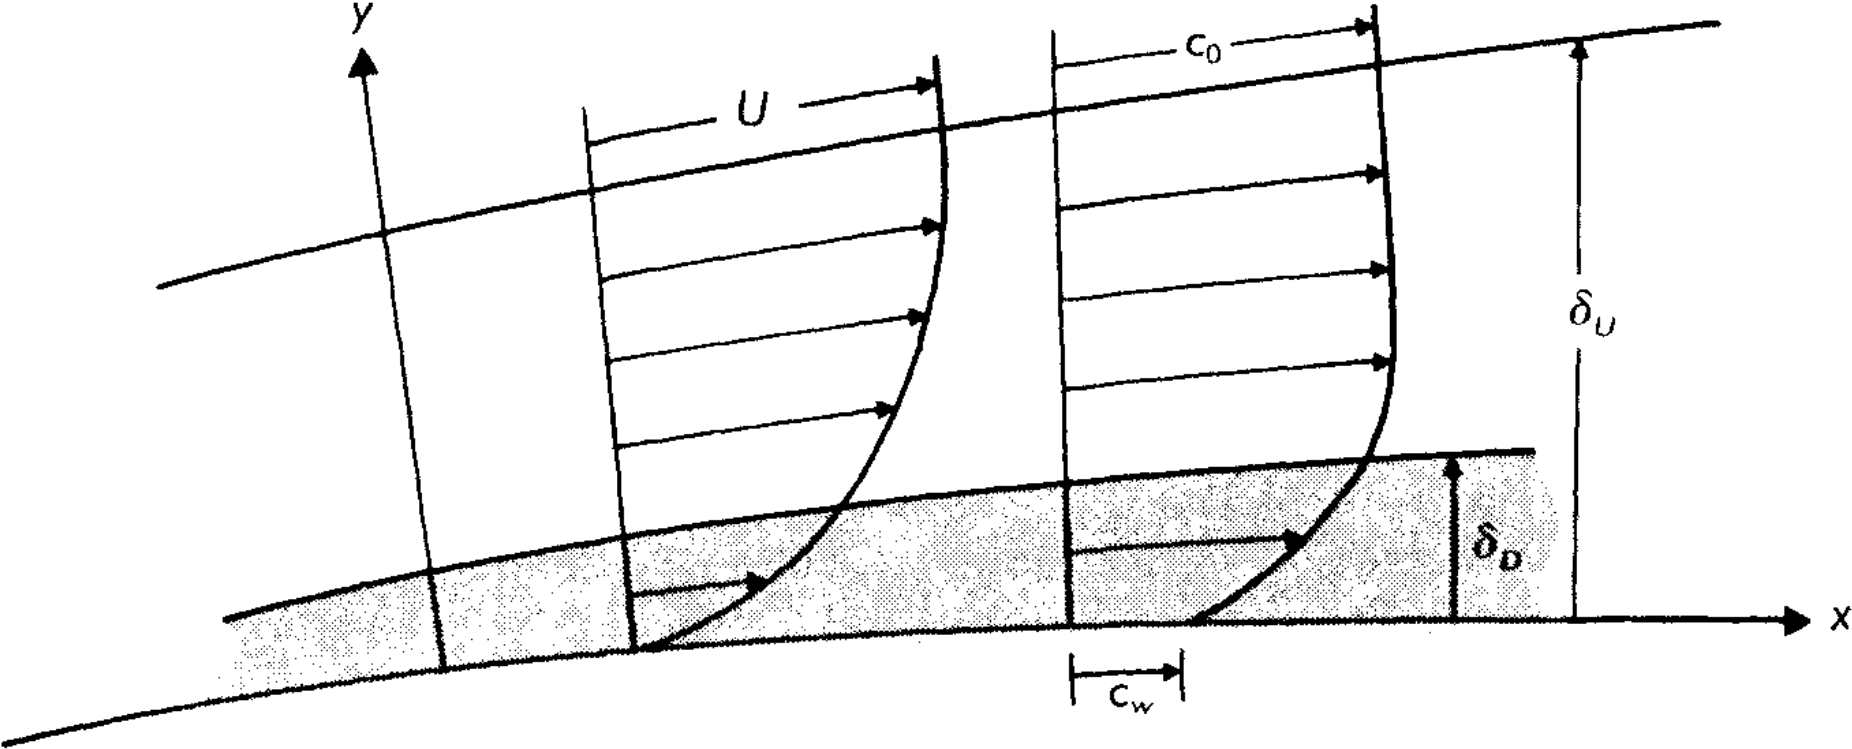
\includegraphics[width=.7\textwidth]{pic/visc_diff_layers}
  \caption{\label{fig:visc_diff_layers}%
    Вязкостный и диффузионный слои;
    $\delta_U$ и $\delta_D$ --- их толщины соответственно
  }

\end{figure}



\Subsection{Моделирование в микрофлюидике}
Математическое моделирование микрофлюидных систем может быть использовано для:
\begin{itemize}
  \item предсказания свойств чипа до его производства,
    что удешевляет разработку конечного функционального изделия,

  \item интерпретации данных, получаемых с помощью чипа,

  \item определения свойств исследуемой системы
    (путём решения обратных задач).

\end{itemize}
% TODO больше о моделировании

\subsubsection*{Решение системы~\eqref{eq:main}}
Как правило, говорить об аналитическом решении системы~\eqref{eq:main}
не приходится и система решается численно, методами конечных элементов.

Методы конечных элементов --- семейство методов численного решения
уравнений математической физики, состоящие в разбиении расчётной области
на конечное число подобластей --- конечных элементов,
на которых выбираются базисные функции,
равные нулю всюду кроме своих элементов
(или конечного их числа, смотря что иметь в виду под элементом),
а решение ищется в виде линейной комбинации этих функций.
Это проиллюстрировано на рисунке~\ref{fig:basis_functions_FEM_illustration1d}.

\begin{figure}
  \centering
  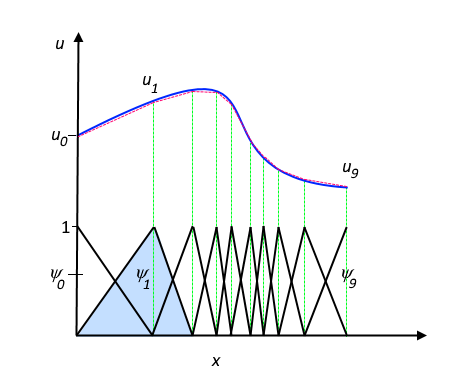
\includegraphics[width=.5\textwidth]{pic/basis_functions_FEM_illustration1d}
  \caption{\label{fig:basis_functions_FEM_illustration1d}%
    Аппроксимация функции $u\left(x\right)$ линейной комбинацией
    финитных базисных функций $\psi_{i=\overline{0,9}}\left(x\right)$
    (\href{https://cdn.comsol.com/cyclopedia/finite-element-method/plot-using-discretization.png}
          {www.comsol.com/multiphysics/finite-element-method})
  }

\end{figure}

На примере уравнения Пуассона
\begin{equation} \Delta u = f\left(\vb x\right) \label{eq:poisson_strong}\end{equation}
выберем гильбертово пространство $H$ и будем искать
$u: \Omega \rightarrow \mathbb{R} \in H: \forall \psi \in H$
\begin{equation}
  \int\limits_\Omega \psi \Delta u d\vb x =
  \int\limits_{\partial\Omega} \psi \nabla u \cdot \vb{dS} -
    \int\limits_\Omega \nabla\psi \cdot \nabla u d\vb x =
  \int\limits_\Omega \psi f d\vb x.
\label{eq:poisson_weak}
\end{equation}
Здесь~\eqref{eq:poisson_weak} --- слабая (вариационная) формулировка,
$\psi$ --- пробная функция.

При применении методов конечных элементов в качестве $H$ выбирается линейная
оболочка набора финитных бызисных функций $\psi_i$, о которых речь шла выше.
Решение ищется в виде их линейной комбинации $u = \sum_i u_i\psi_i$
Уравнение~\eqref{eq:poisson_weak} заменяется на систему (по индексу $j$)
\begin{equation}
  \sum_i u_i \left(
    \int\limits_{\partial\Omega} \psi_j \nabla \psi_i \cdot \vb{dS} -
    \int\limits_\Omega \nabla\psi_j \cdot \nabla \psi_i d\vb x
  \right) =
  \int\limits_\Omega \psi_j f d\vb x,
\label{eq:poisson_FEM}
\end{equation}
что можно записать в виде
\begin{equation}
  \hat{A}\vb u = \vb f,
\label{eq:poisson_FEM_obscure}
\end{equation}
где $\vb u$ --- столбец с элементами $u_i$,
$\vb f$ --- столбец с элементами $f_i = \int_\Omega\psi_i f d\vb x$,
$\hat{A}$ --- матрица с элементами $A_{ij} =
  \int_{\partial\Omega} \psi_i \nabla \psi_j \cdot \vb{dS} -
    \int_\Omega \nabla\psi_i \cdot \nabla \psi_j d\vb x$.
Таким образом, численное решение уравнения Пуассона методами конечных элементов
запишется как
\begin{equation}
  u\left(\vb x\right) =
    \sum_i\left[\hat{A}^{-1}\vb f\right]{}_i\psi_i\left(\vb x\right).
\end{equation}

В случае с уравнением теплопроводности
\begin{equation}
  \frac{\partial u}{\partial t} - \Delta u =
    f\left(\vb x, t, u\left(\vb x, t\right)\right)
\label{eq:heat_strong}
\end{equation}
имеет смысл (для уменьшения вычислительных затрат)
искать приближённое решение в виде
$u = \sum_i u_i\left(t\right)\psi_i\left(\vb x\right)$
(вместо $\sum_i u_i\psi_i\left(\vb x, t\right)$).
В таком случае уравнение~\eqref{eq:heat_strong} будет приближаться
(аналогично~\eqref{eq:poisson_FEM})
\begin{equation}
  \sum_i \frac{\partial u_i}{\partial t} \int\limits_\Omega \psi_i\psi_j d\vb x +
    \sum_i u_i \left(
      -\int\limits_{\partial\Omega} \psi_j \nabla \psi_i \cdot \vb{dS} +
      \int\limits_\Omega \nabla\psi_j \cdot \nabla \psi_i d\vb x
    \right) =
  \int\limits_\Omega \psi_j f_t d\vb x,
\label{eq:heat_FEM}
\end{equation}
где $f_t\left(\vb x\right) =
  f\left(\vb x, t, \sum_i u_i\psi_i\left(\vb x\right)\right)$.
Выражение $\partial u_i/\partial t$ заменится конечной разностью, например
\begin{equation}
  \frac{\partial u_i}{\partial t} \approx
    \frac{u_i\left(t + \Delta t\right) - u_i\left(t\right)}{\Delta t},
\label{eq:heat_time_forward_finite_difference}
\end{equation}
в таком случае подстановка $u_i = u_i\left(t\right)$ в~\eqref{eq:heat_FEM}
позволит явно выразить $u_i\left(t + \Delta t\right)$ через $u_i\left(t\right)$:
\begin{equation}
  \vb u\left(t + \Delta t\right) =
    \vb u\left(t\right) +
      \Delta t\hat{\Psi}^{-1} \left(\hat{A}\vb u\left(t\right) +
                                    \vb f_t\left(\vb u\left(t\right)\right)\right),
\label{eq:heat_FEM_explicit}
\end{equation}
где $\hat{\Psi}$ --- матрица с элементами $\Psi_{ij} = \int_\Omega\psi_i\psi_j d\vb x$,
$\vb u(t)$ --- столбец с элементами $u_i\left(t\right)$,
$\vb f_t\left(\vb u\left(t\right)\right)$ ---
  столбец с элементами $f_{t,i} = \int_\Omega\psi_i f_t d\vb x$,
$\hat{A}$ определена так же, как и для уравнения Пуассона выше.

Если пользоваться~\eqref{eq:heat_time_forward_finite_difference},
и принять $u_i = u_i(t + \Delta t)$ в~\eqref{eq:heat_FEM},
то полученное уравнение будет задавать
$u_i\left(t + \Delta t\right)$ как функцию $u_i\left(t\right)$ неявно.
Неявная постановка вычислительно более затратна, но
оказывается необходимой при решении так называемых \emph{жёстких} систем,
которые часто встречаются при наличии химических реакций
(когда уравнение теплопроводности является, по сути, уравнением диффузии).

Методы конечных элементов реализованы, например, в программном обеспечении
COMSOL Multiphysics\texttrademark\ (далее --- COMSOL),
которое и используется в этой работе.

\subsubsection*{Решение обратных задач}
Как было сказано выше, для определения характеристик исследуемых систем
могут решаться обратные задачи.
Если решение прямой задачи состоит в предсказании поведения системы,
про которую всё известно, то решение обратной задачи состоит в оценке
параметров системы по её поведению.

Обратные задачи математически формулируются как задачи оптимизации ---
минимизации некоторого функционала ошибки $Q:\mathbb{P}\rightarrow\mathbb{R}_+$,
где $\mathbb{P}$ --- пространство параметров,
$\mathbb{R}_+ = \left\{x\in\mathbb{R}|x\leqslant0\right\}$.
Если $\vb x_{t}$ --- состояние системы в момент времени $t$, а
$\vb f\left(t,\vb p\right)$ --- предсказание состояния системы с параметрами
$\vb p \in \mathbb{P}$ в момент времени $t$, то
типичным функционалом ошибки
\begin{equation}
Q\left(\vb p\right) =
  \frac{\sum\limits_{t\in T}\left(\vb f\left(t,\vb p\right) - \vb x_t\right){}^2}
       {\left|T\right|},
\end{equation}
где $T$ --- конечное множество времён.
Данный функционал гладкий, что позволяет для его оптимизации использовать
градиентные методы; если аналитическое выражение для градиента не известно,
он может быть в каждой точке оценён численно.

Например, при адсорбции из идеально перемешанного реактора
согласно кинетике действующих масс, соответствующей изотерме Ленгмюра,
поверхностная концентрация адсорбированного аналита
в момент времени $t$ будет равна
\begin{equation}
  \gamma\left(t\right) = f\left[c\right]\left(\Gamma_0, k_f, k_r, t\right),
\end{equation}
где $c:T\rightarrow\mathbb{R}_+$ --- концентрация аналита в растворе в зависимости от времени,
$\Gamma_0$ --- поверхностная концентрация сайтов связывания,
$k_f$ и $k_r$ --- кинетические константы, характеризующие адсорбцию и десорбцию,
$f$ --- решение уравнения
$\dot{\gamma} = k_f \left(\Gamma_0-\gamma\right) c - k_r \gamma$,
которое может быть получено численно.
Пусть теперь в каждый момент времени известна концентрация $c\left(t\right)$
(например, через реакционную камеру протекают растворы с известными концентрациями)
и имеется линейный по поверхностной концентрации адсорбировавшегося аналита
сигнал с прибора $s\left(t\right) = \alpha\gamma\left(t\right)$.
Тогда для сигнала будет справедливо
\begin{equation}
\begin{cases}
  \dot{s} = \alpha\dot{\gamma} = k_f \left(s_{\max} - s\right) - k_r s \\
  s = s_t = s_0 + \int\limits_{t_0}^{t} \dot{s} dt = g(t, s_{\max}, k_f, k_r) \\
\end{cases}
\end{equation}
и по набору значений $s_{t \in T}$ можно будет оценить параметры
$s_{\max}$, $k_f$ и $k_r$,
как это сделано в~\cite{bib:FULLTEXT_inverse_example} (рис.~\ref{fig:FULLTEXT_inverse_example}).

\begin{figure}
  \centering
  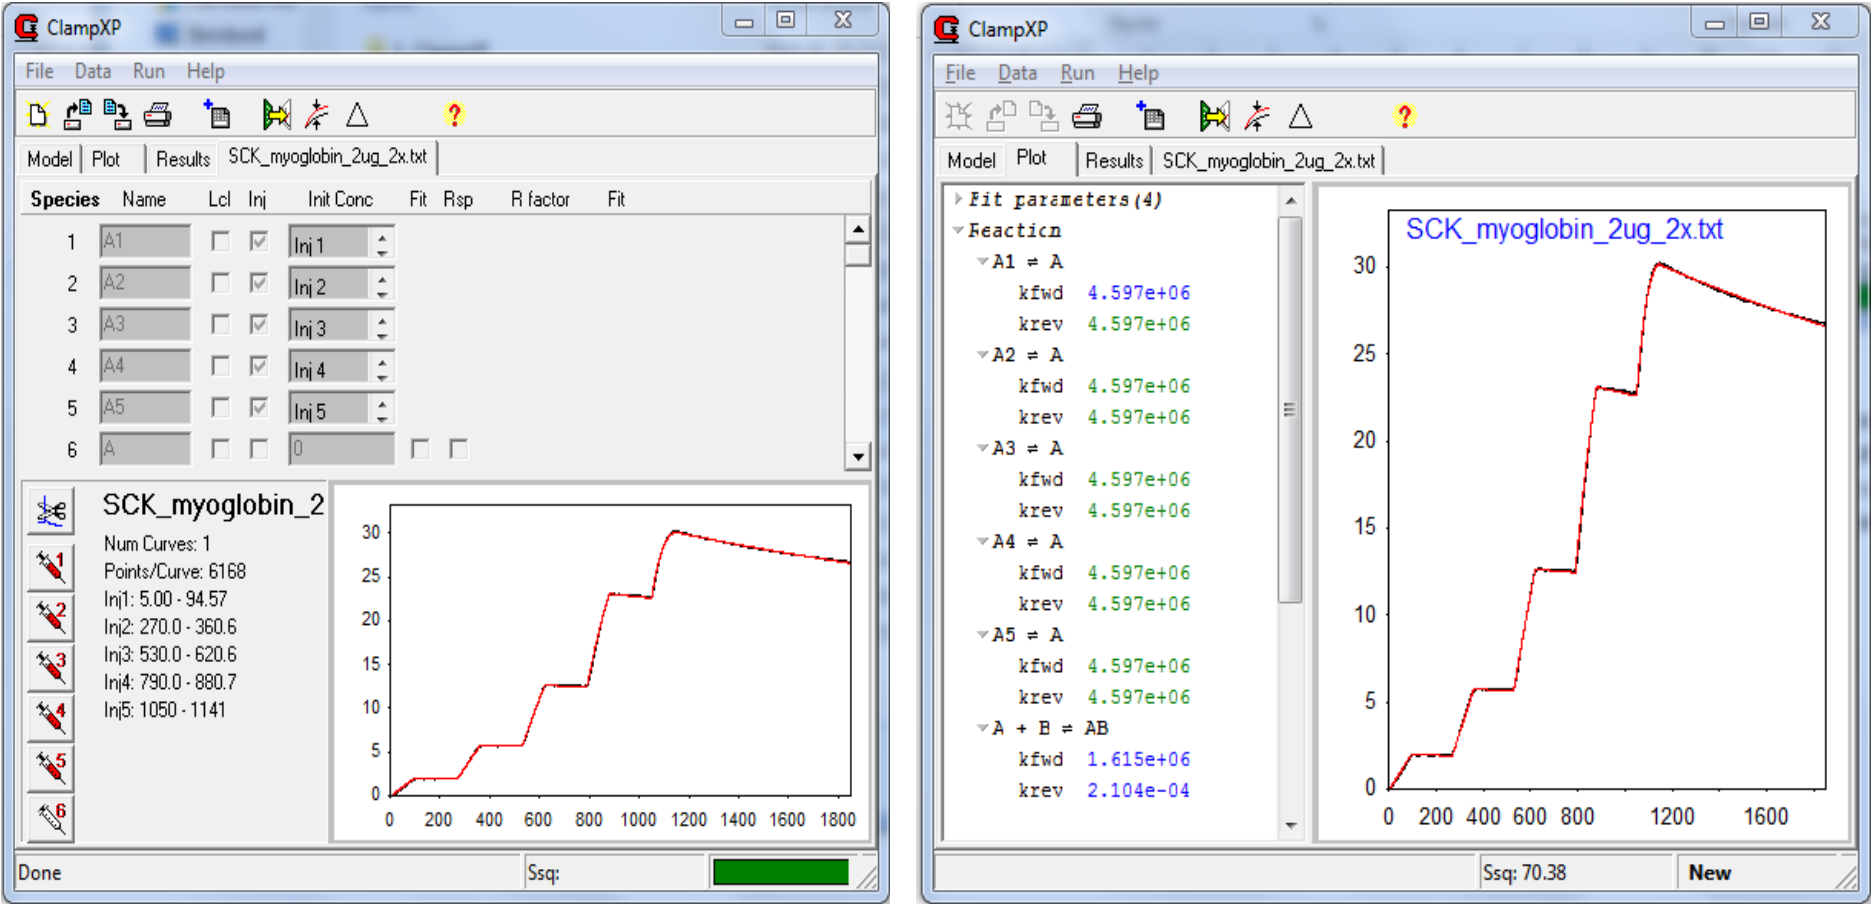
\includegraphics[width=.8\textwidth]{pic/FULLTEXT_inverse_example}
  \caption{\label{fig:FULLTEXT_inverse_example}%
    Решение обратной задачи в~\cite{bib:FULLTEXT_inverse_example}
    с помощью ClampXP:
    в левом окне задаётся концентрация аналита в растворе от времени,
    в правом окне внизу слева полученные оценки кинетических констант
  }

\end{figure}


% TODO обратные задачи

% TODO каплегенераторы

\Section{Основное содержание}

\Subsection{Адсорбция на поверхность бесконечно широкого канала с одним видом сайтов связывания}

\subsubsection*{Физическое описание}
Имеется раствор вещества A (аналит),
в котором так же может присутствовать вещество B (примесь).
На плоской поверхности канала,
вдоль которой течёт этот раствор,
имеются сайты связывания.
Это проиллюстрировано на рисунке~\ref{fig:flat_wide_illustration}
(см. также~\ref{fig:visc_diff_layers}).

\begin{figure}[h]
  \centering
  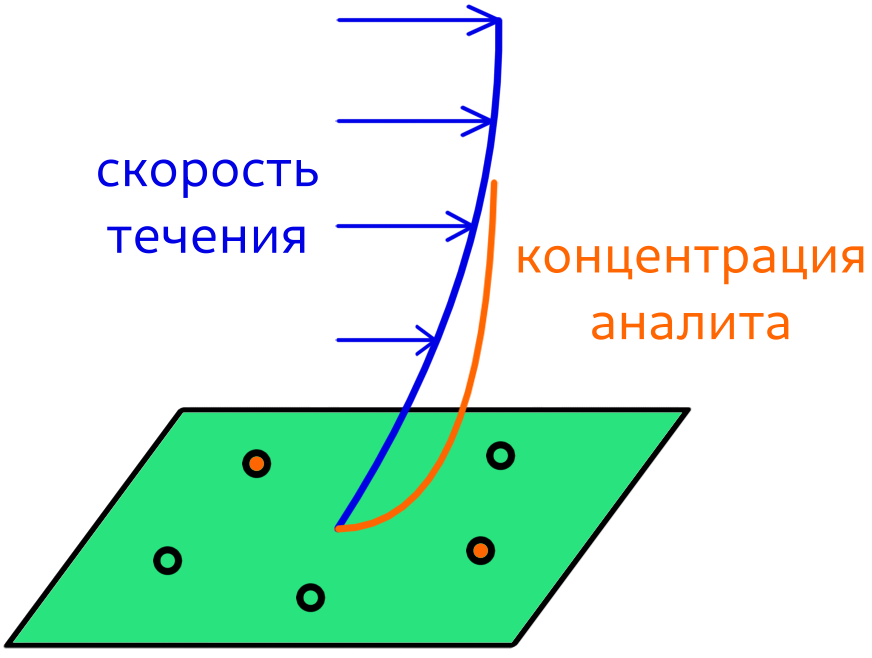
\includegraphics[width=.4\textwidth]{pic/flat_illustration}
  \caption{\label{fig:flat_wide_illustration}%
    Иллюстрация к задаче об адсорбции на поверхность;
    цветные кривые изображают зависимость
    скорости течения и концентрации аналита
    от расстояния до поверхности;
    оранжевые круги --- сайты связывания, связавшиеся с аналитом,
    салатовые --- свободные сайты связывания
  }

\end{figure}

Кинетика связывания соотвестсвует изотерме Ленгмюра
(см.~\eqref{eq:Langmuir_multi_many_kin}).

\subsubsection*{Одномерная постановка без примеси}
В качестве расчётной области берётся отрезок с длиной $\delta_D$
диффузионного слоя (см.~\eqref{eq:diffusion_layer}).
На одном конце отрезка происходит химическая реакция
связывания веществ из раствора с сайтами связывания на поверхности,
на другом --- фиксируется концентрация $c_0$.

Изначально концентрация веществ в растворе однородна (всюду равна $c_0$) и
все сайты связывания свободны (на поверхности нет связвашегося аналита).

Толщину вязкостного слоя $\delta_U$ можно представить в виде
\begin{equation}
  \label{eq:viscous_layer_alpha}
  \delta_U = \alpha\sqrt{\frac{U\nu}{L}},
\end{equation}
где $\alpha$ --- безразмерный параметр порядка единицы.
В этой части в формуле~\eqref{eq:diffusion_layer} для расчёта $\delta_D$
знак $\sim$ заменён на знак равенства, а
$\alpha$ в~\eqref{eq:viscous_layer_alpha} принимается равным $\sqrt{2}$,
последнее будет обосновано ниже.

Параметры задачи:%
скорость течения раствора равна $U = 0.1\text{мм}/\text{с}$,
характерная длина $L = 2\text{мм}$,
вязкость раствора равна вязкости воды (\SI{20}{\celsius}).
В качестве аналита принимается стрептавидин,
его коэффициент диффузии оценён в $D = 8\cdot10^{-5}\text{мм}^2/\text{с}$,
а молекулярная масса --- в $m_{\text{str}} = 60\text{кДа}$.
Кинетические константы были приняты равными
$k_f = 10^7\left(\text{М}\cdot\text{с}\right)^{-1}$
и $k_r = 10^{-7}\text{с}^{-1}$ в соответствии с оценкой из~%
\cite{bib:biotin_streptavidin_kinetics}
кинетики связывания комплекса биотин-стрептавидин.
Поверхностная концентрация сайтов связывания принята равной
$\Gamma = 3.85\cdot10^{-8}\text{моль}/\text{м}^2 = 0.023\text{нм}^{-2} = 1/\left(43.5\text{нм}^2\right)$
(связывание со всеми сайтами будет соответствовать примерно
70\% заполнения всей поверхности молекулами стрептавидина).

На рисунке~\ref{fig:flat_wide_onecomp_onedim_probe_distrib}
представлены результаты симуляций со значениями концентрации
$c_0 = 0.1 \text{мг}/\text{мл}$ и $c_0 = 0.01 \text{мг}/\text{мл}$.
Во втором случае диффузионный слой успевает истощиться до насыщения поверхности,
после 100--200 секунд с нулевого момента времени адсорбции лимитируется
максимальной возможной скоростью диффузии через диффузионный слой
$j_{\text{max}} = D c_0 / \delta_D$.

\begin{figure}
  \centering
  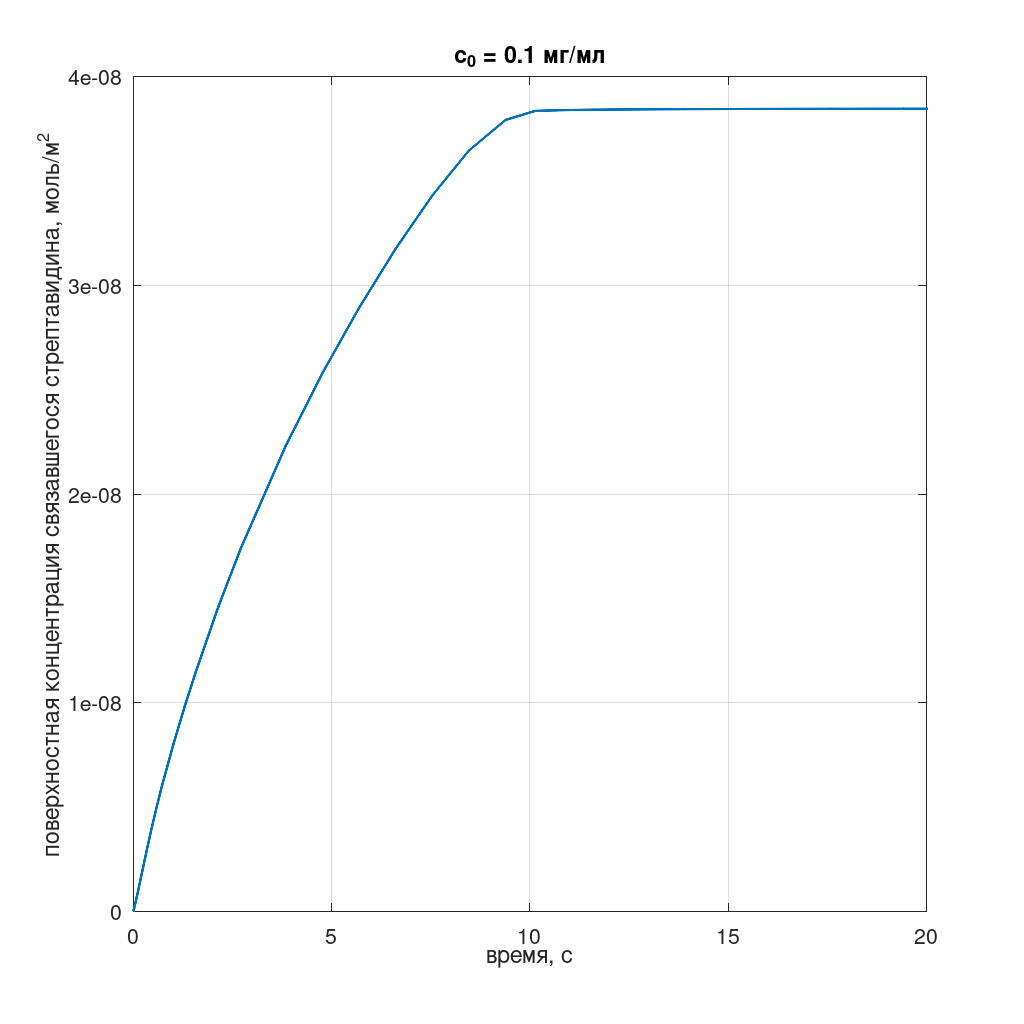
\includegraphics[width=.5\textwidth]{pic/flat_wide_onecomp_onedim_ref_probe}%
  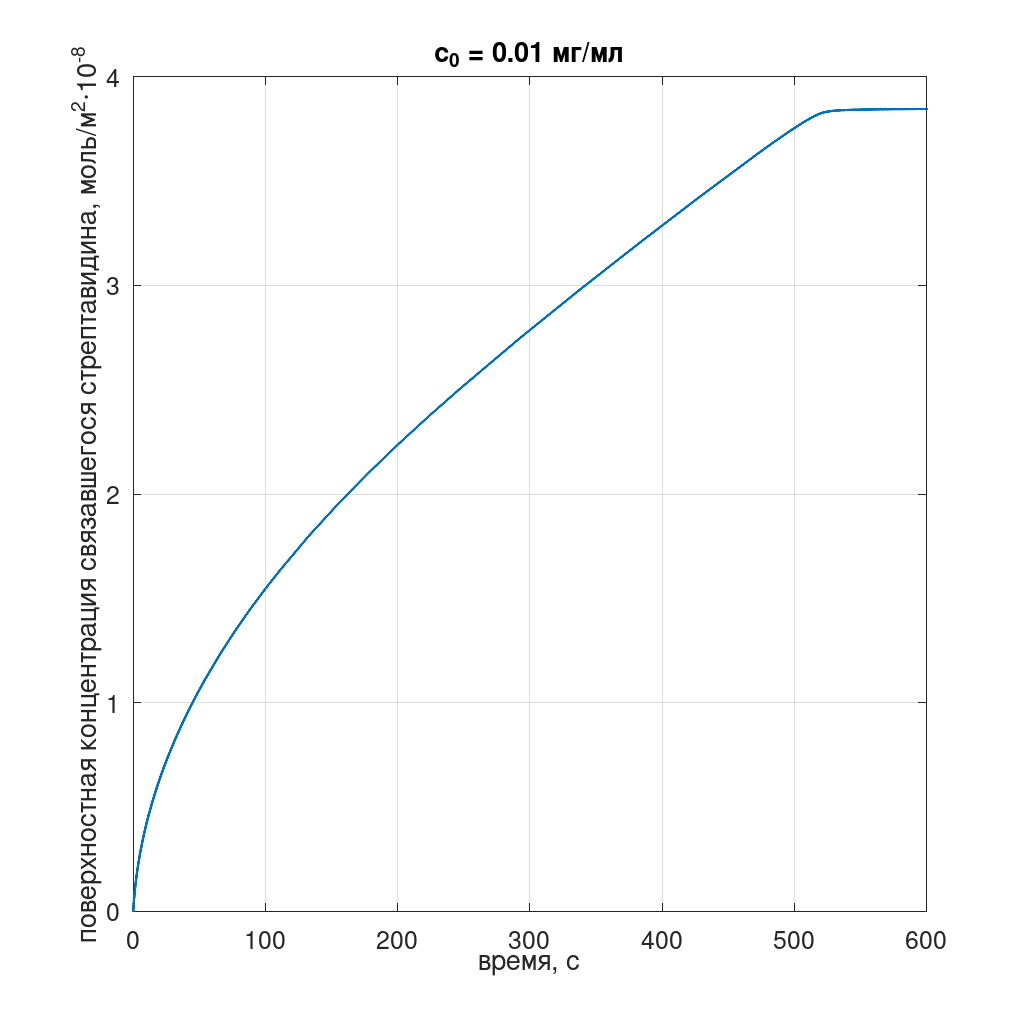
\includegraphics[width=.5\textwidth]{pic/flat_wide_onecomp_onedim_dil10_probe}

  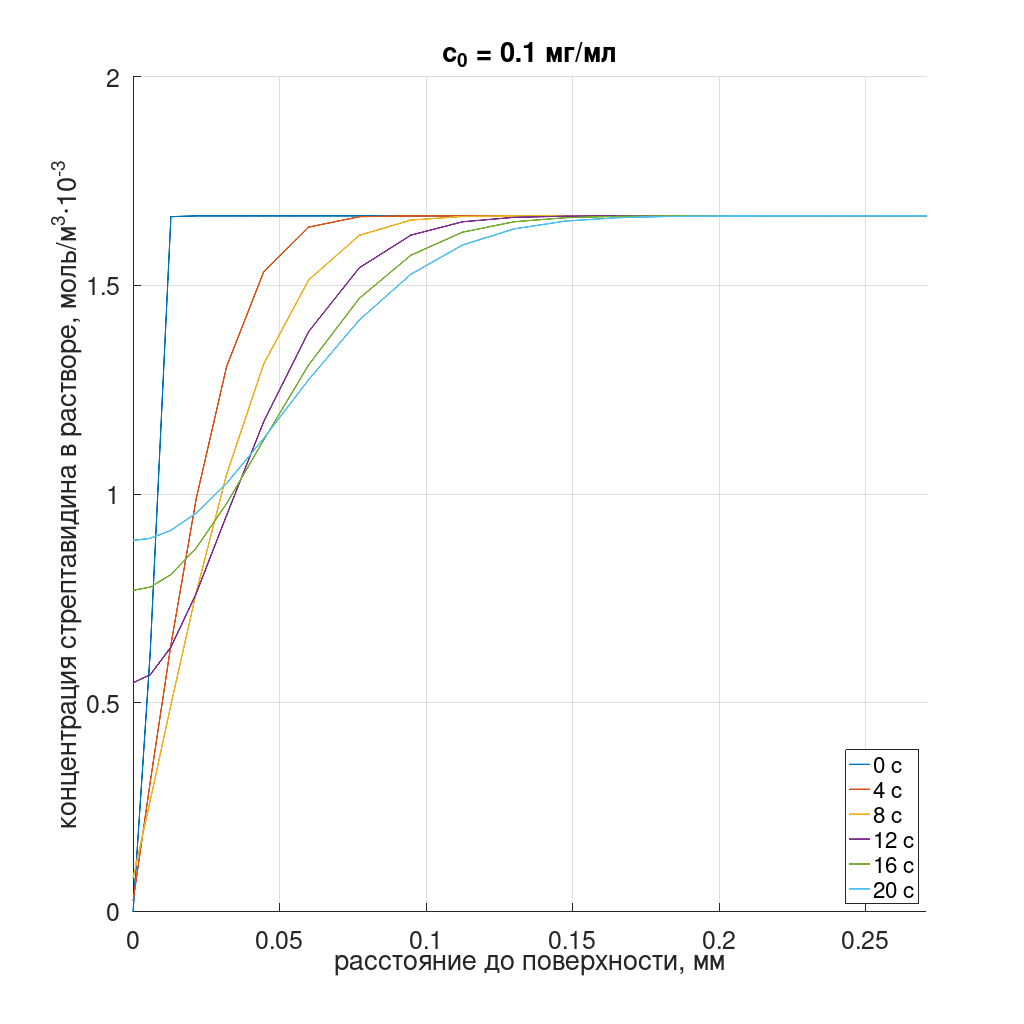
\includegraphics[width=.5\textwidth]{pic/flat_wide_onecomp_onedim_ref_distrib}%
  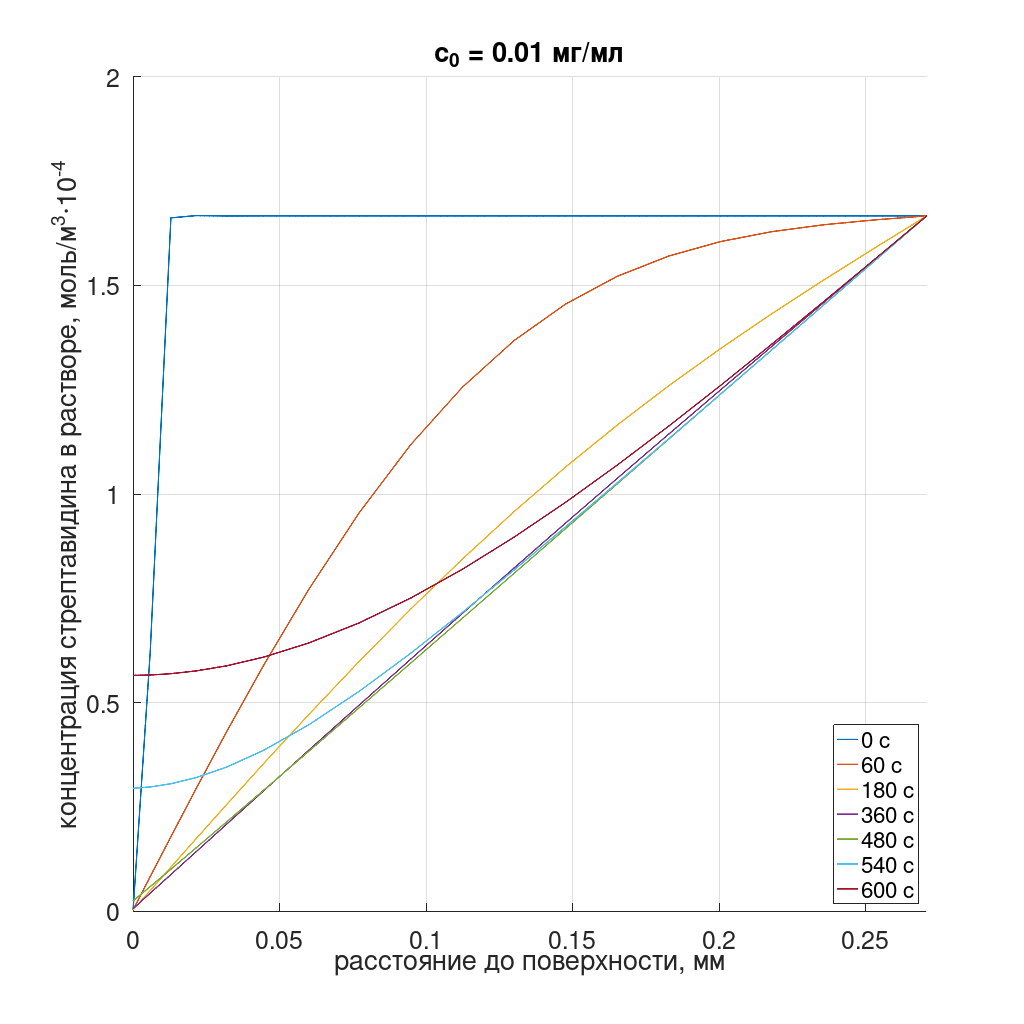
\includegraphics[width=.5\textwidth]{pic/flat_wide_onecomp_onedim_dil10_distrib}

  \caption{\label{fig:flat_wide_onecomp_onedim_probe_distrib}%
    Результаты расчётов в одномерной задаче об адсорбции
    на стенку бесконечно широкого канала;
    \textbf{сверху:} зависимость концентрации связвашегося стрептавидина от времени,
    \textbf{снизу:} пространственное распределение стрептавидина по объёму раствора;
    \textbf{слева:} $c_0 = 0.1 \text{мг}/\text{мл}$,
    \textbf{справа:} $c_0 = 0.01 \text{мг}/\text{мл}$
  }

\end{figure}

\subsubsection*{Одномерная постановка с примесью}
Относительно стрептавидина, задача идентична предыдущей
с $c_0 = 0.01 \text{мг}/\text{мл}$.
Добавляется примесь с начальной и граничной концентрациями
$c_1 = 100 c_0$.
Константа диссоциации примеси и сайтов связывания равна
$K_{B,d} = 10^{-3} \text{М}$,
для кинетической константы $k_{B,f}$ рассматриваются значения
$k_{B,f} = 10^3 \left(\text{М} \cdot \text{с}\right)^{-1}$ и
$k_{B,f} = 10^4 \left(\text{М} \cdot \text{с}\right)^{-1}$.
Полученные зависимости поверхностных концентраций
стрептавидина, примеси и свободных сайтов связывания от времени
приведены на рисунке~\ref{fig:flat_wide_twobulk_paramsweep}.

\begin{figure}
  \centering
  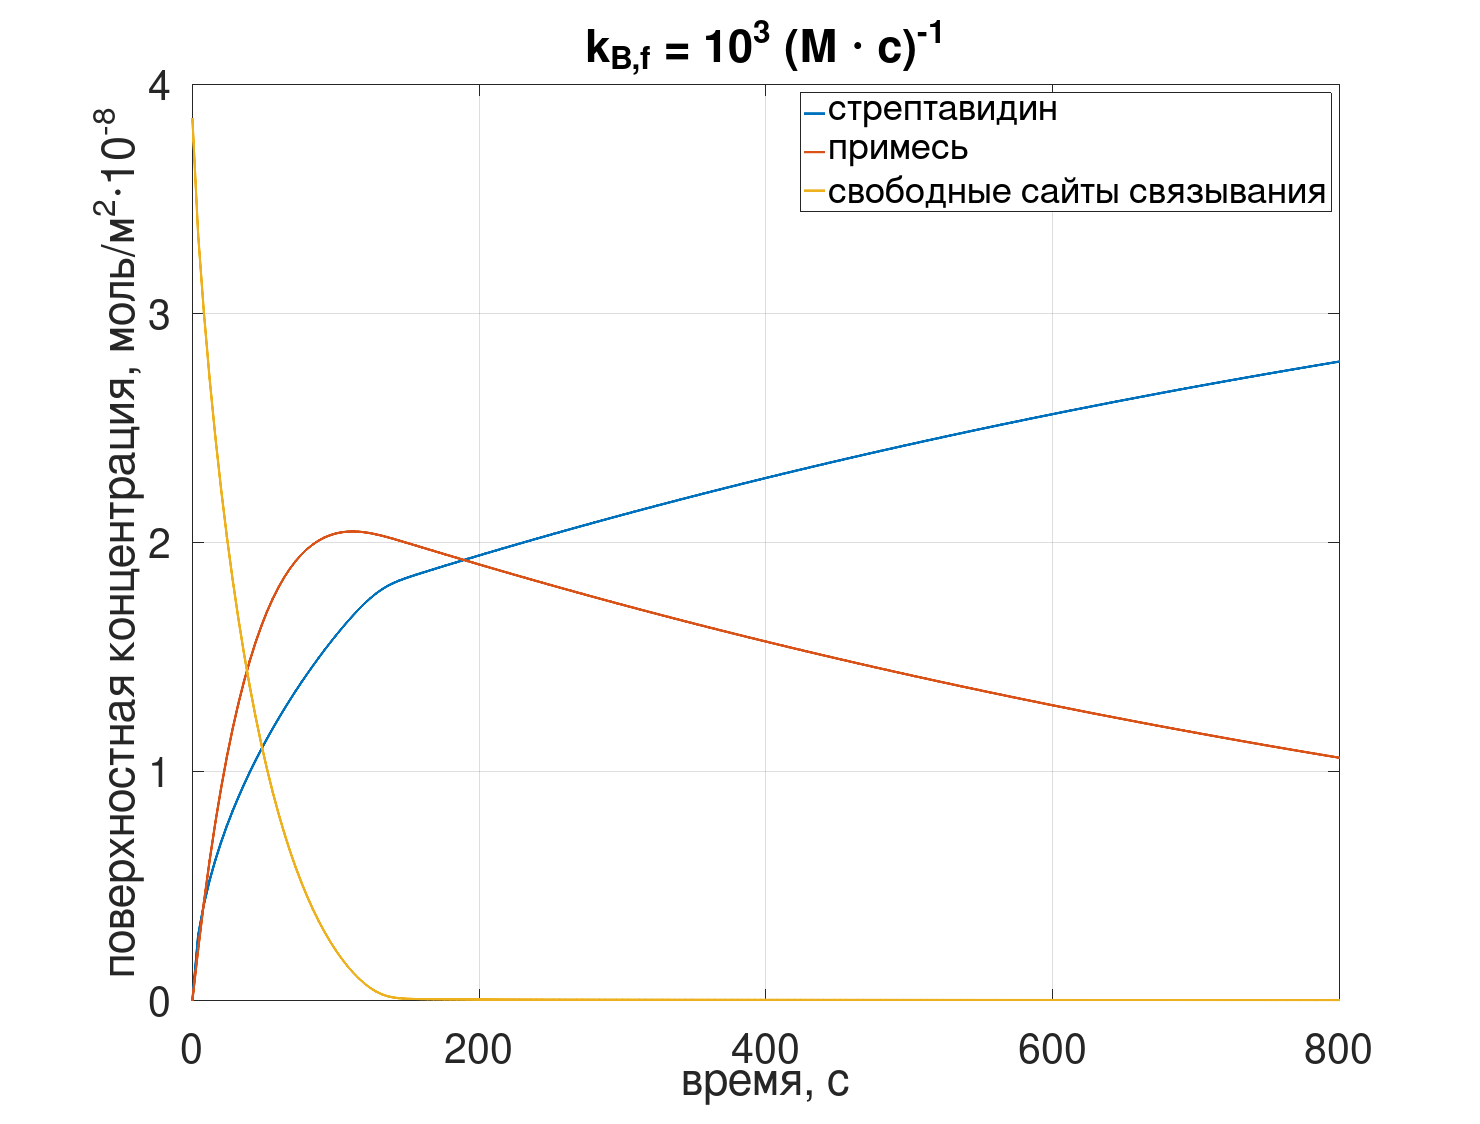
\includegraphics[width=.6\textwidth]{pic/flat_wide_two_bulk_paramsweep_3}
  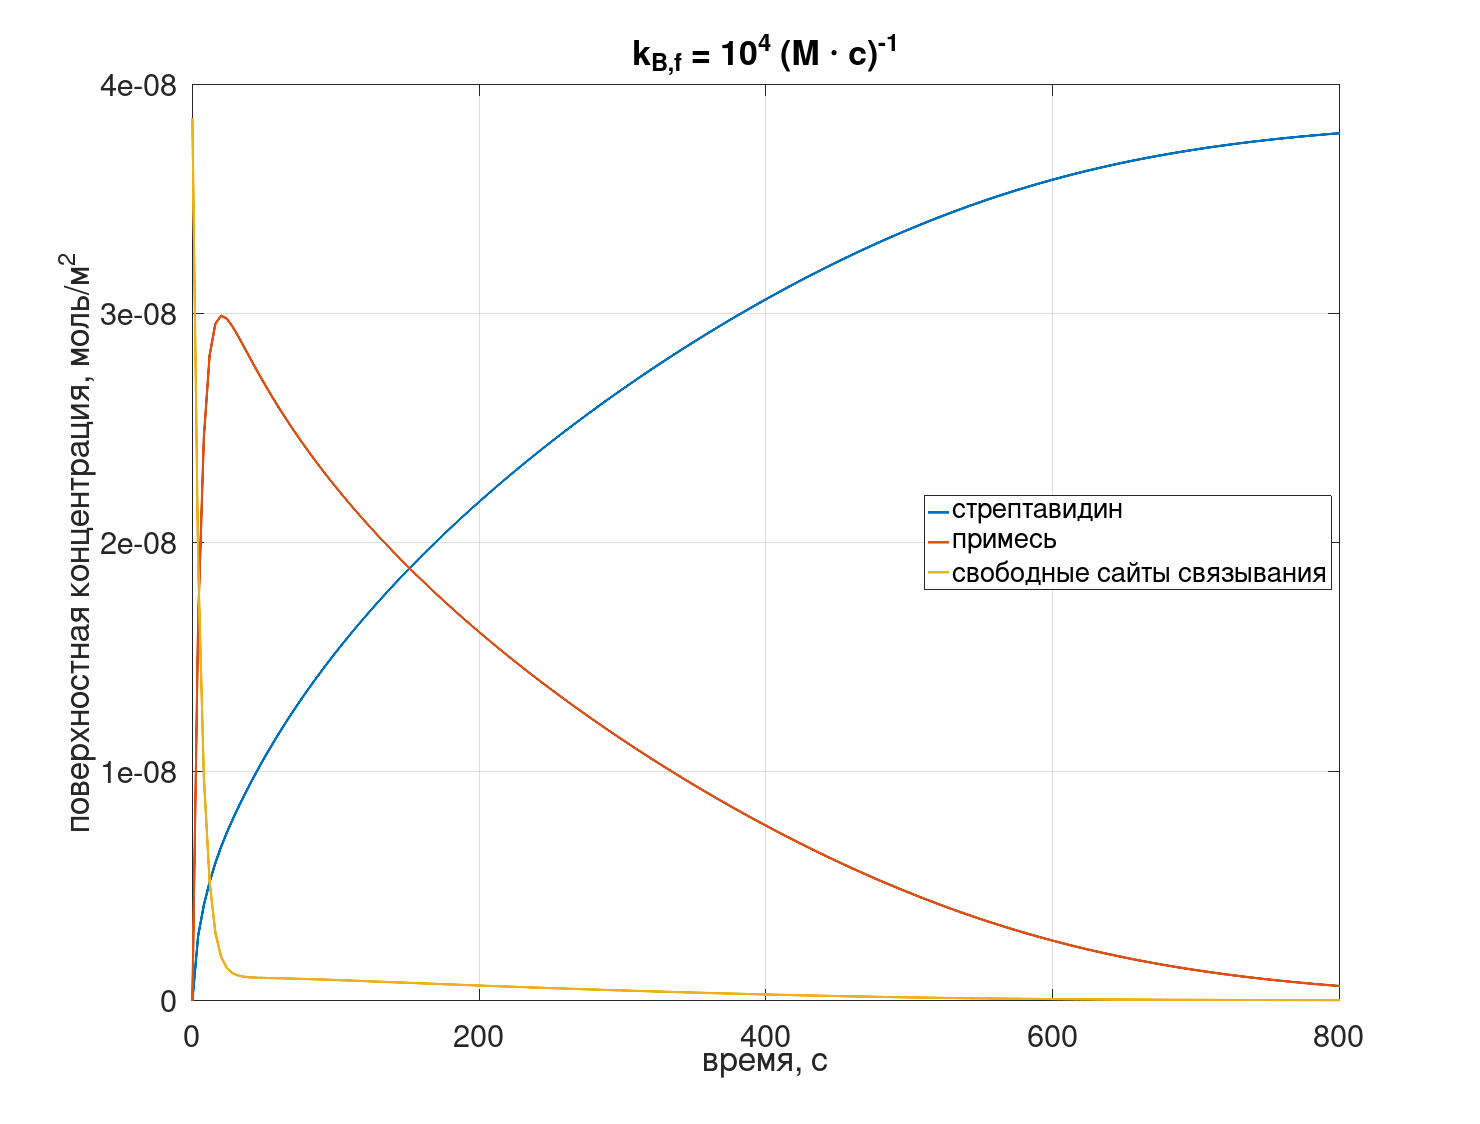
\includegraphics[width=.6\textwidth]{pic/flat_wide_two_bulk_paramsweep_4}

  \caption{%
    \label{fig:flat_wide_twobulk_paramsweep}%
    Одномерная постановка задачи об адсорбции на стенку бесконечно широгоко канала
    при наличии примеси;
    зависимость поверхностных концентраций стрептавидина, примеси и
    свободных сайтов связывания от времени
  }
\end{figure}



\subsubsection*{Двумерная постановка (без примеси)}

Расчётная область представляет из себя прямоугольник со сторонами
$a = 3 L$ и $b = 2 \delta_U$.
Значение $\delta_U$ расчитывается по формуле~\eqref{eq:viscous_layer}
с заменой знака $\sim$ на $=$.
Значения всех параметров те же, что и в одномерной постановке;
$c_0 = 0.01 \text{мг}/\text{мл}$.

На поверхности канала (сторона $a$, нижняя граница расчётной области)
сайты связывания расположены на отрезке
длиной $L = 2 \text{мм}$, отстоящем от обоих концов рассматриваемой части поверхности канала
на расстоянии $L$ (см. рис.~\ref{fig:flat_wide_plate_illustration} сверху слева).
Вдоль левой границы расчётной области скорость потока равна
$U = 0.1 \text{мм}/\text{с}$ и направлена вдоль поверхности канала.
На верхней границе расчётной области концентрация зафиксирована и равна
$c_0 = 0.01 \text{мг}/\text{мл}$.

На рисунке~\ref{fig:flat_wide_plate_illustration} изображены
распределение концентрации стрептавидина в части объёма раствора
в пределах $2 \delta_D$ от стенки канала
(в прямоугольнике со сторонами $a = 3 L$ и $b = 2 \delta_D$)
в моменты времени
$140\text{с}$ и $350\text{с}$,
а сверху --- пространственное распределение скорости течения раствора
во всей расчётной области.
Этот рисунок подтверждает справедливость оценок
\eqref{eq:viscous_layer} и \eqref{eq:diffusion_layer}
толщин $\delta_U$ и $\delta_D$ вязкостного и диффузионного слоёв.

\begin{figure}
  \centering
  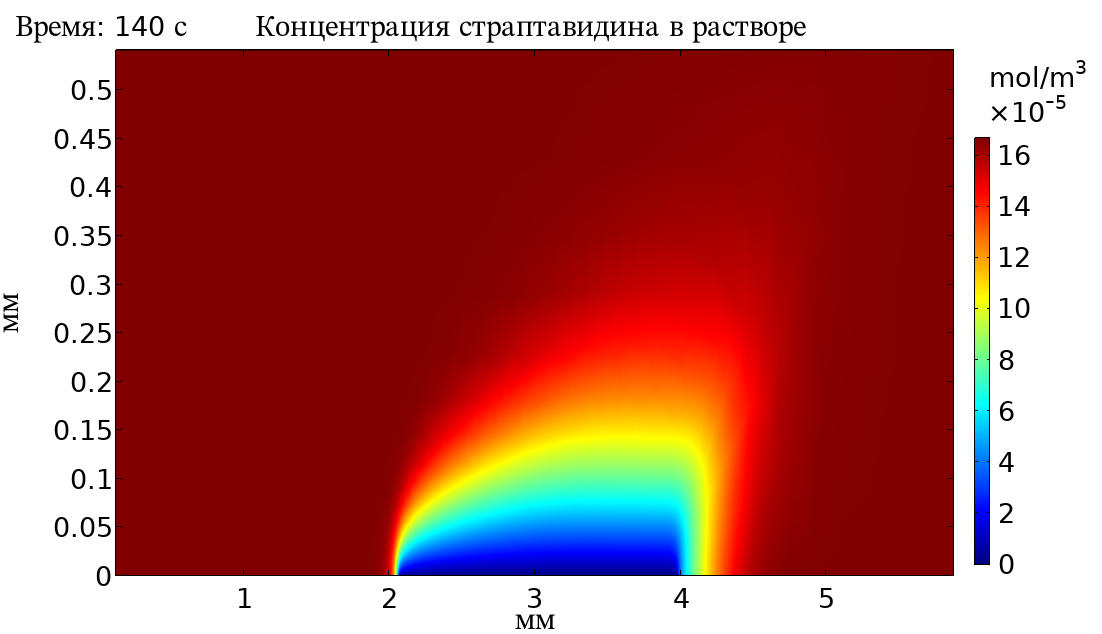
\includegraphics[width=.5\textwidth]{pic/flat_wide_onecomp_plate_concentration_140s}%
  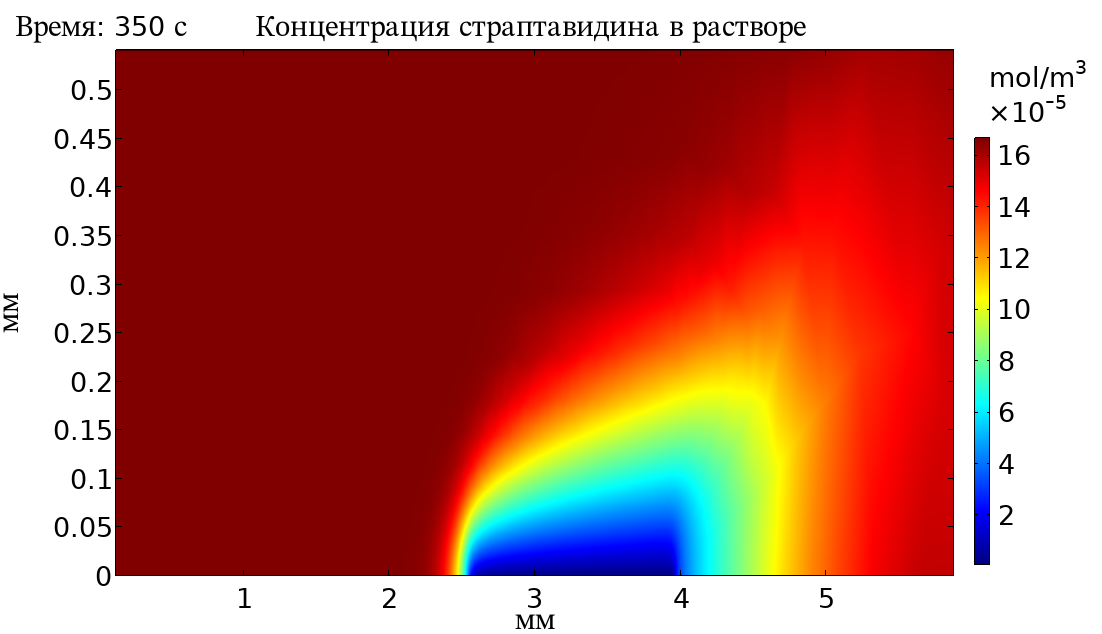
\includegraphics[width=.5\textwidth]{pic/flat_wide_onecomp_plate_concentration_350s}

  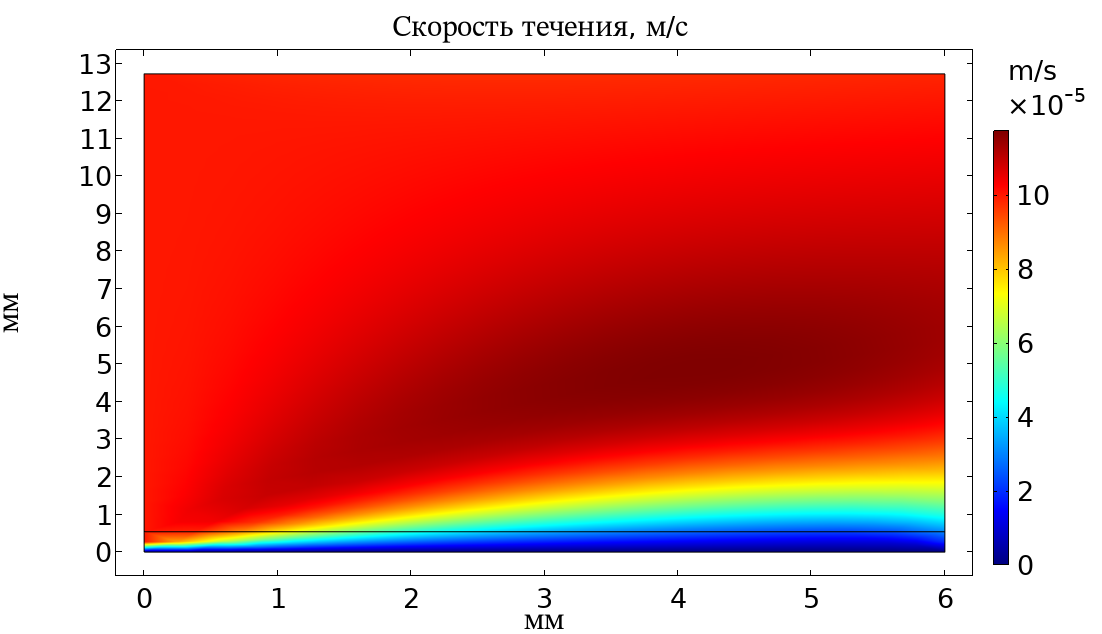
\includegraphics[width=.6\textwidth]{pic/flat_wide_onecomp_plate_velocity}

  \caption{\label{fig:flat_wide_plate_illustration}%
    Иллюстрация к двумерной постановке задачи об адсорбции
    на стенке бесконечно широкого канала;
    \textbf{сверху:} концентрация стрептавидина в растворе
    спустя 140с (слева) и 350с (справа) после нулевого момента времени,
    \textbf{снизу:} распределение скорости течения в объёме раствора
  }
\end{figure}

На рисунке~\ref{fig:flat_wide_onecomp_alphas}
представлено сравнение зависимости средней концентрации
связвашегося стрептаведина в данной (двумерной) постановке
от времени с аналогичными зависимостями в одномерной постановке
при значениях параметра
$\alpha \in \left\{ 1, \sqrt{2}, 2 \right\}$
(см.~\eqref{eq:viscous_layer_alpha}).
Этот рисунок говорит как о разумности применения одномерного приближения
с оценками~\eqref{eq:viscous_layer} и~\eqref{eq:diffusion_layer},
так и о разумности выбора $\alpha = \sqrt{2}$.

\begin{figure}
  \centering
  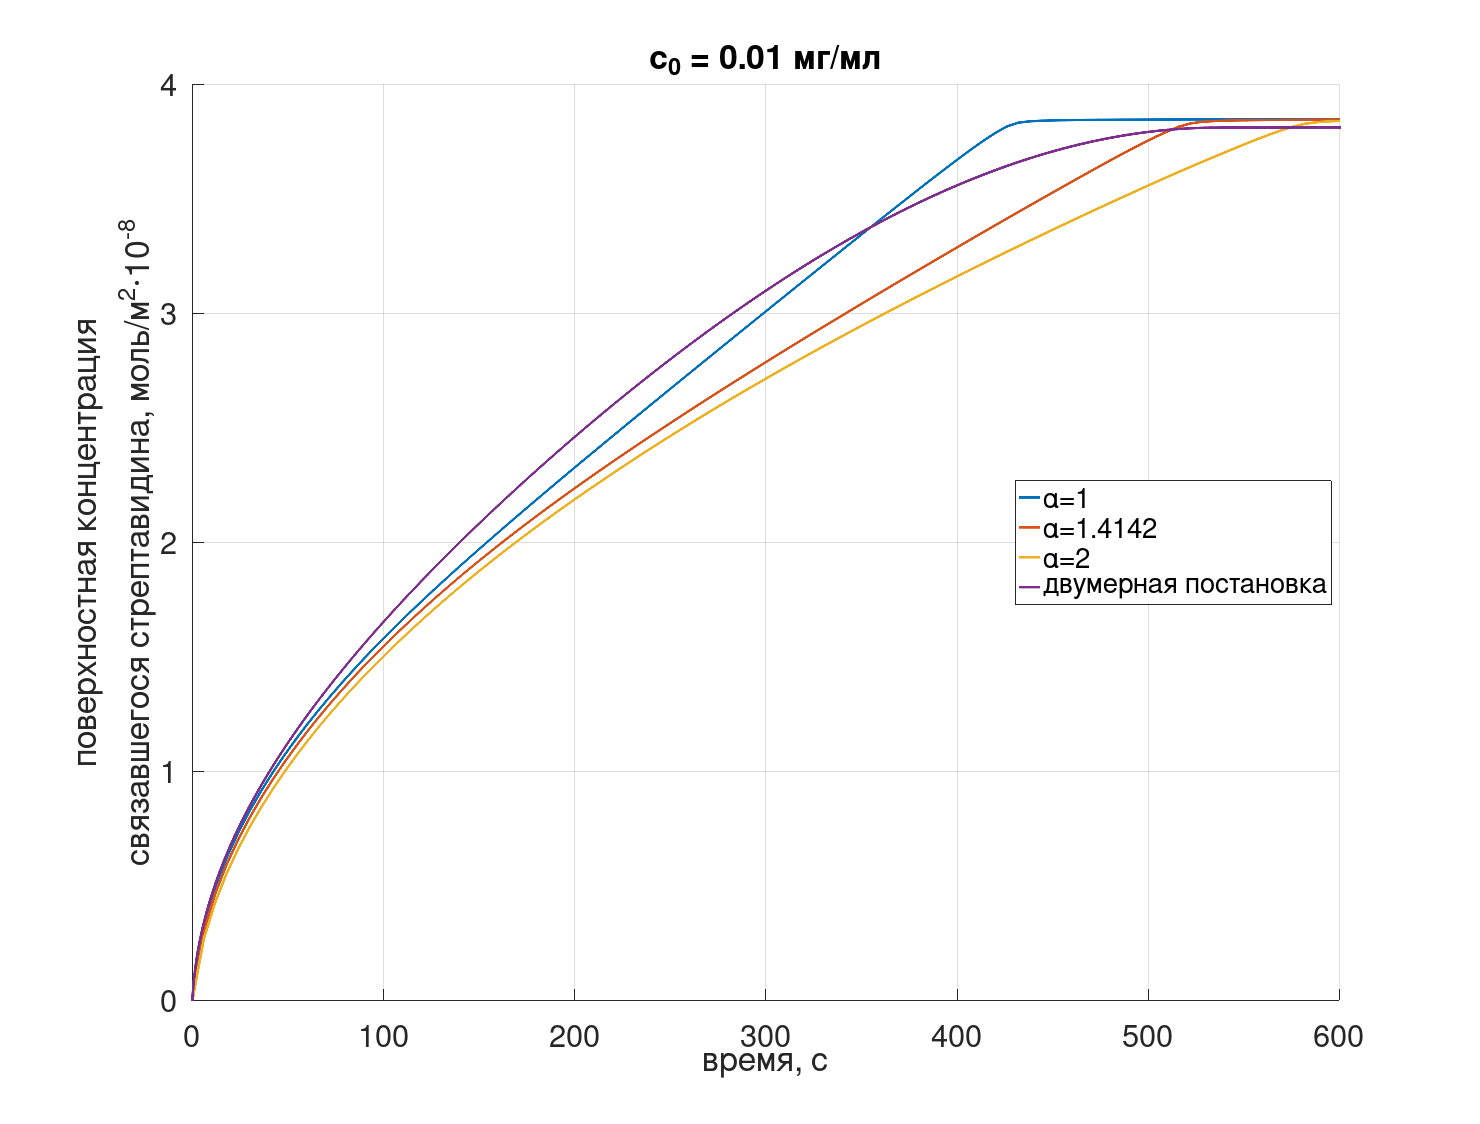
\includegraphics[width=.7\textwidth]{pic/flat_wide_onecomp_streptalphas}

  \caption{%
    \label{fig:flat_wide_onecomp_alphas}%
    Сравнение зависимости средней концентрации
    связвашегося стрептаведина в двумерной постановке
    от времени с аналогичными зависимостями в одномерной постановке
    при значениях параметра
    $\alpha \in \left\{ 1, \sqrt{2}, 2 \right\}$
  }

\end{figure}

% TODO показать слияние размера сетки на результаты

\Subsection{Адсорбция на поверхность бесконечно широкого канала с двумя видами сайтов связывания}

\subsubsection*{Одномерная постановка}

Задача во многом похожа на предыдущую, но теперь имеются 2 вида сайтов связывания:
A и B, соответствующие специфическому и неспецифическому связыванию.
Химические константы равны
$k_{A,f} = 3 \cdot 10^4 \left(\text{М}\cdot\text{с}\right)^{-1}$,
$k_{B,f} = 10^3 \left(\text{М}\cdot\text{с}\right)^{-1}$,
$K_{A,a} = 10^8 \text{М}^{-1}$, $K_{B,a} = 10^6 \text{М}^{-1}$.
Это соответствует примерно кинетике связывания белка A и белка G с
иммуноглобулином G, взятой из~\cite{bib:protein_a_b_ig_g},
с понижением $k_{B,f} = k_{G,f}$ и $K_{B,a} = K_{G,a}$ на порядок.
Коэффициент диффузии принимается равным
$D = 2 \cdot 10^{-5} \text{мм}^2/\text{с}$,
а масса молекулы аналита --- $m = 50\text{кДа}$.
Суммарная поверхностная концентрация сайтов связывания равна
$\Gamma = 4.37 \cdot 10^{-8} \text{моль}/\text{м}^2 = 0.026 \text{нм}^{-2} = 1/\left(38.5\text{нм}^2\right)$.
Доли $a$ и $b$ сайтов A и B варьируются, но всегда $a+b=1$
(количество сайтов A $\Gamma_A = a\Gamma$, сайтов B --- $\Gamma_B = b\Gamma$).
Примеси нет.

Начальные условия выставляются неоднородные,
см. рис.~\ref{fig:flat_wide_ramp_ic}.
Граничные условия меняются во времени: первые $1000\text{с}$
на границе фиксируется концентрация $c_0$,
следующие $7000\text{с}$ --- нулевая концентрация, что соответствует отмывке
неспецифически адсорбировавшегося вещества.

\begin{figure}
  \centering
  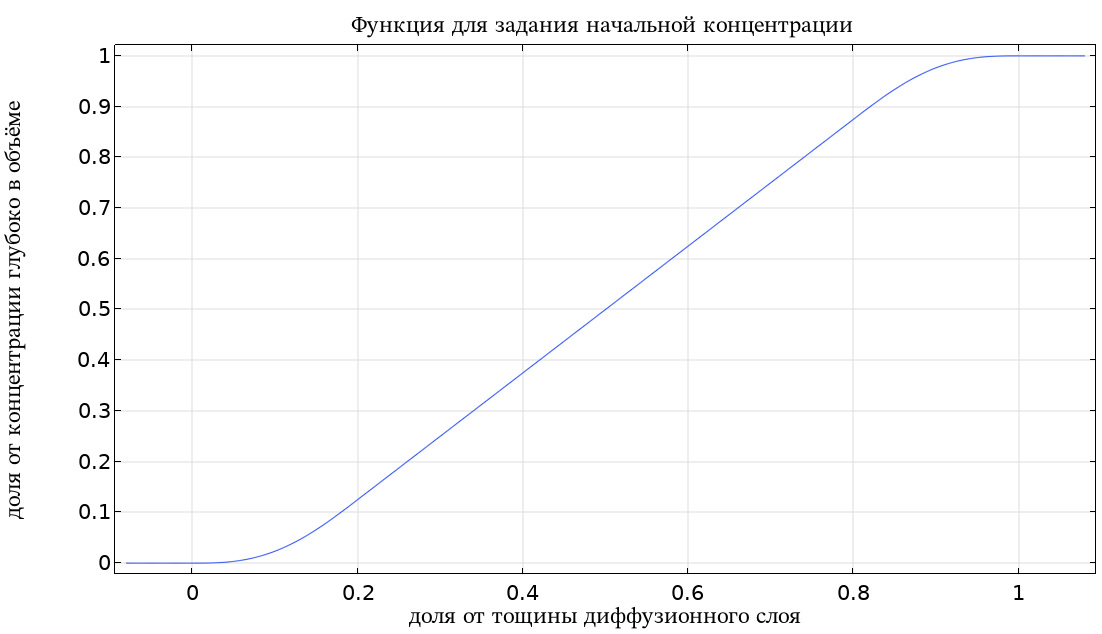
\includegraphics[width=.7\textwidth]{pic/wide_two_surf_ramp}
  
  \caption{%
    \label{fig:flat_wide_ramp_ic}%
    Иллюстрация к неоднородным начальным условиям в одномерной постановке
    задачи об адсорбции на поверхность канала
  }

\end{figure}

На рисунке~\ref{fig:flat_wide_two_surf_example} предствлена зависимость
поверхностной концентрации аналита, связавшегося специфически (с сайтами A),
неспецифически (с сайтами B), и их суммы при значении параметра $a = 0.5$,
т. е. при одинаковом количестве сайтов A и B.
Благодаря меньшему сродству аналита к сайтам B, чем к сайтам A, отмывка
от неспецифически адсорбировавшегося вещества возможна
(с сохранием значимой части специфически адсорбировавшегося).

\begin{figure}
  \centering
  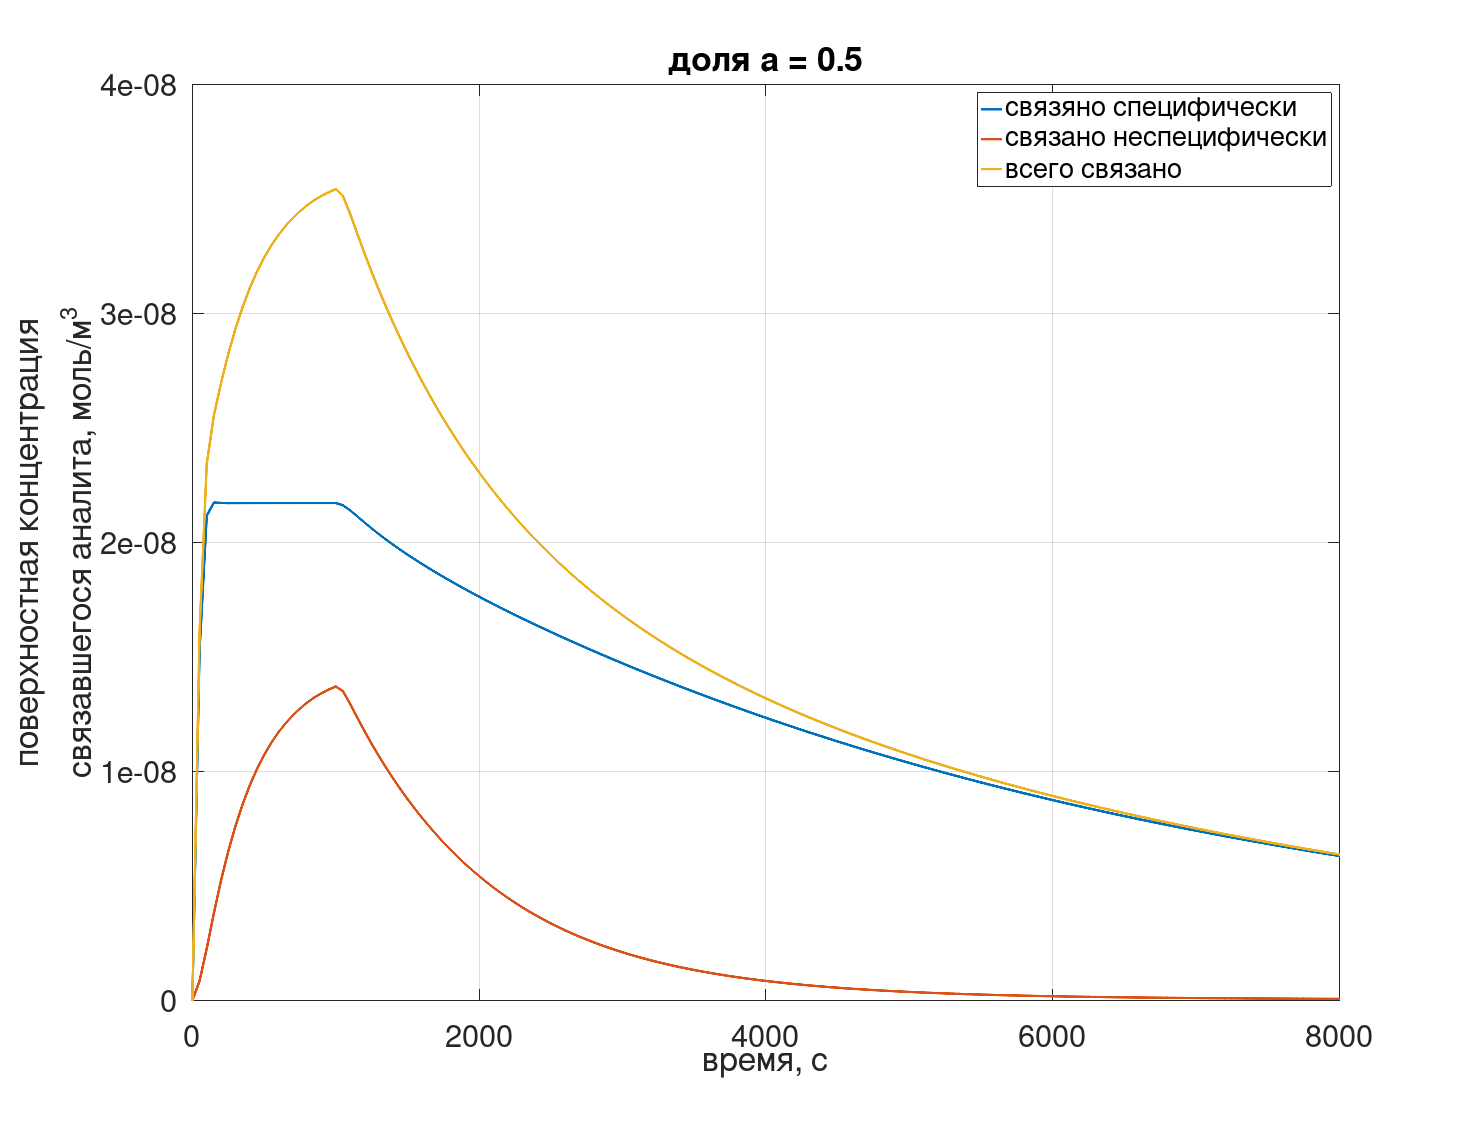
\includegraphics[width=.7\textwidth]{pic/flat_wide_twosurf_example}

  \caption{%
    \label{fig:flat_wide_two_surf_example}%
    Задача об одномерной адсорбции на стенку бесконечно широкого канала
    при наличии неспецифической адсорбции;
    зависимость поверхностной концентрации аналита,
    связавшегося специфически, неспецифически, и суммарно;
    доля сайтов A $a = 0.5$, т. е. сайтов A и B поровну
  }

\end{figure}

На рисунке~\ref{fig:wide_two_surf_fracs_a_sum} представлены зависимости
поверхностной концентрации связавшегося специфически (с сайтами A) и
связвашегося всего (суммарно с сайтами A и B)
аналита от времени при различных долях $a$ сайтов A.
Видно, что количество специфически связавшегося аналита существенно сильнее
зависит от параметра $a$, чем общее количество связавшегося аналита,
что может быть важно, если регистрируемый прибором сигнал пропорционален
суммарному количеству связвашегося аналита или
показания прибора иначе зависят от неспецифической адсорбции аналита.
Это наблюдение говорит о возможной важности отмывки.
Количество неспецифически связавшегося аналита не изображено,
т. к. это сделало бы рисунок нечитаемым.

\begin{figure}
  \centering
  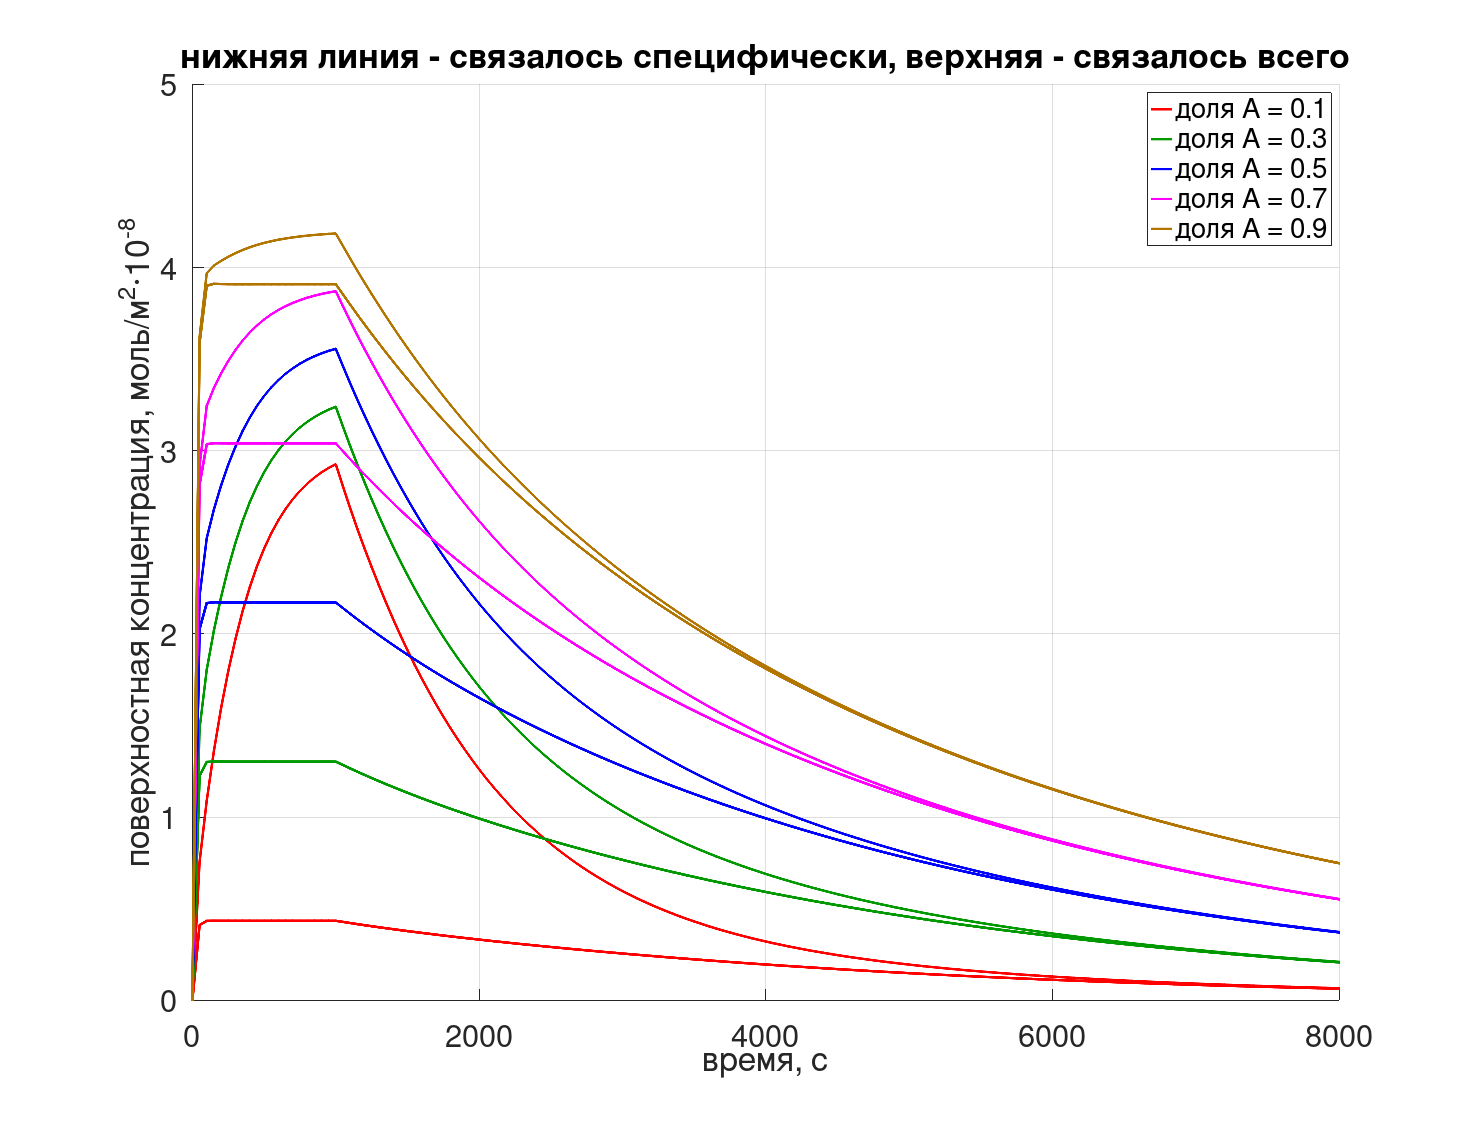
\includegraphics[width=.7\textwidth]{pic/flat_wide_twosurf_fracs_a_sum}

  \caption{%
    \label{fig:wide_two_surf_fracs_a_sum}%
    Задача об одномерной адсорбции на стенку бесконечно широкого канала
    при наличии неспецифической адсорбции;
    цветом объединены графики зависимости специфически адсорбировавшегося и
    суммарно адсорбировавшегося аналита при фиксированном параметре $a$~---
    доле сайтов специфического связывания от общего количества сайтов связывания
    (включая неспецифические)
  }

\end{figure}


\subsubsection*{Двумерная постановка}


\Subsection{Адсорбция на поверхность канала конечной ширины с двумя видами сайтов связывания}

% TODO невозможность уменьшить расчётную область


% \Subsection{Адсорбция на мембране}

\Subsection{Адсорбция на микросферах}

\subsubsection*{Физическое описание}

\subsubsection*{В покое}

\subsubsection*{В потоке}

% \Subsection{Каплегенераторы}



\Section{Материалы и методы}

\Section{Результаты и обсуждение}

\Section{Заключение}

\Section{Выводы}


\bibliographystyle{plain}
\bibliography{bibliography,bib/springer_handbook.bib,bib/phys_chem_hydro_layers.bib}




\end{document}
